\chapter{Distribuciones bidimensionales: Correlación y Regresión lineal}
\chaptermark{Estad. 2-D: Correlación y Regresión}

%*************************************************************************
% ATENcION: por cambio ordenación temas, 2 <--> 3, las imagenes de 3.Prob. 
%están en imagenes02 y las imágenes de 2.Estad 2D están en imagenes03.
%*************************************************************************


\begin{tikzpicture}
	\fill [left color=red!50, right color=teal!50] (0,0) rectangle (6.5,.1);
	\fill [left color=teal!50, right color=green!50] (6.5,0) rectangle (11.5,.1);
	\end{tikzpicture}




\section[Distribuciones estadísticas bivariantes]{Distribuciones estadísticas bivariantes \sectionmark{Distribuciones 2-Dim}}
 \sectionmark{Distribuciones 2-Dim}



\begin{definition}


	

\begin{multicols}{2}
 
Si de una determinada muestra o población se estudian dos caracteres simultneamente, se obtienen dos series de datos de la forma:
 
\begin{table}[H]
\centering
\begin{tabular}{c|cccccc}
\textbf{$x_i$} & $x_1$ & $x_2$ & $x_3$ & $\cdots$ & $\cdots$ &  \\ \cline{1-6}
\textbf{$y_i$} & $y_1$ & $y_2$ & $y_3$ & $\cdots$ & $\cdots$ &  \\ \cline{1-6}
\textbf{$n_i$} & $n_1$ & $n_2$ & $n_3$ & $\cdots$ & $\cdots$ & $\ \to \Sigma N$
\end{tabular}
\end{table}
 
\end{multicols} 


 
Donde $x_i$ e $y_i$ son las variables estadísticas correspondientes a las carateristicas observadas y $n_i$ es la frecuencia absoluta de cada pareja de datos $(x_i,y_i)$, es decir, $n_i$ es el número de veces que se repite el par $(x_i,y_i)$.
 
\vspace{2mm}  A la lista de estos pares ordenados de datos con sus respectivas frecuencias se le llama \textbf{\emph{variable estadística bidimensional}}, $\ \boldsymbol{ (x_i, \ y_i; \ n_i)}$.

\vspace{2mm} La frecuencia relativa del par $(x_i,y_j)$ es $f_{i j} = n_{i j}/N$ , donde $N$ denota el número total de pares observados.

\vspace{2mm} Las \textbf{\emph{variables marginales}}\footnote{Las distribuciones marginales son las distribuciones unidimensionales que nos informan del número de observaciones para cada valor de una de las variables, prescindiendo de la información sobre los valores de las demás variables.} $X$ e $Y$ toman los valores $\{x1,x2,...,xm\},$  $\{y1,y2,...,yr\}$ para ciertos $m$, $r$, respectivamente, y la variable bidimensional $(X,Y)$ tomará los valores $\{(xi,yj)\}\ 1\le i \le m,\ 1 \le j \le r$.
 
\end{definition}
 

\begin{example}

Se muestran algunos ejemplos de variables bidimensionales:

\begin{itemize}

\item $(X,Y)$ (sexo, color del ojos); $X$ cualitativa; $Y$ cualitativa.

\item $(X,Y)$ (nivel de estudios, lustros en la empresa); $X$ cualitativa; $Y$ cuantitativa (discreto -años-).

\item $(X,Y)$ (número de hermanos, número de hijos); $X$ cuantitativa (v.e. discreta); $Y$ cuantitativa (v.e. discreta).

\item $(X,Y)$ (peso, estatura); $X$ cuantitativa (v.e. continua); $Y$ cuantitativa (v.e. continua).

En este tema nos interesarán las variables estadísticas bidimensionales en que ambas sean cuantitativas.
\end{itemize}
\end{example}

\begin{theorem}
.	Nótese que:

$$\displaystyle \sum_{i=1}^m \ \sum_{j=1}^r\ n_{ij}\ = \ N;\qquad 	\qquad \qquad\sum_{i=1}^m \ \sum_{j=1}^r\ f_{ij}\ = \ 1$$
\end{theorem}



\subsection{Distribuciones de frecuencias}
	


\begin{definition}
.	Se define la \textbf{frecuencia (absoluta) marginal} del valor $x_i$ como la suma de las frecuencias correspondientes a los pares $(x_i,y_j)$, para $1 \le  j \le  r$:
	

Análogamente se define la frecuencia (absoluta) marginal del valor $y_j$:

$$n_{x_i}=\displaystyle \sum_{j=1}^r\ n_{ij}; \qquad \qquad \qquad n_{y_j}=\displaystyle \sum_{i=1}^m\ n_{ij}$$
\end{definition}



\begin{theorem}
.	Nótese que $n_{x_i}$ (respectivamente, $n_{y_j}$ ) representa el número de veces que aparece el valor $x_i$ (respectivamente, $y_j$) en el total de pares obtenidos. Se verifica:

$$\displaystyle \sum_{i=1}^m\ n_{x_i}=\sum_{i=1}^m\ \sum_{j=1}^r\ n_{ij}=N; \qquad \qquad \qquad
\sum_{j=1}^r\ n_{x_i}=\sum_{j=1}^r\ \sum_{i=1}^m\ n_{ij} = N$$	
\end{theorem}



	



A partir de las frecuencias absolutas marginales se obtienen las frecuencias relativas marginales.

\begin{definition}
.	 Se definen las \emph{frecuencias relativas marginales} como:

$$\displaystyle f_{x_i}= \dfrac{n_{x_i}}{N};\qquad \qquad \qquad 
f_{y_j}= \dfrac{n_{y_j}}{N}$$	
\end{definition}

\vspace{5mm} %********************************
\begin{theorem}
.	Las frecuencias relativas marginales cumplen:

$$\displaystyle \sum_{i=1}^n\ f_{x_i} \ = \ \dfrac 1 N \ \sum_{i=1}^m\ n_{x_i}=1
\qquad \qquad \qquad   
\sum_{i=1}^n\ f_{y_j} \ = \ \dfrac 1 N \ \sum_{j=1}^r\ n_{y_j}=1$$	
\end{theorem}

\vspace{5mm} %********************************
Todos estos datos se pueden representar en una \colorbox{orange!10}{\textbf{\emph{``tabla de doble entrada''}}} \textcolor{gris}{(así se entenderá mejor)}:


	
\begin{table}[H]
\large
\centering
\begin{tabular}{c|c|c|c|c|c|c}
\cline{1-5}
\multicolumn{1}{|c|}{\textbf{$\ Y \  /  \ X$}} & \textbf{$\boldsymbol{y_1}$} & \textbf{$\boldsymbol{y_2}$} & \textbf{$\cdots$} & \textbf{$\boldsymbol{y_r}$} & \scriptsize{marg X} & \scriptsize{rel X} \\ \hline
\multicolumn{1}{|c|}{\textbf{$\boldsymbol{x_1}$}} & $n_{11}$ & $n_{12}$ & $\cdots$ & $n_{1r}$ & $n_{x_1}$ & $f_{x_1}$ \\ \hline
\multicolumn{1}{|c|}{\textbf{$\boldsymbol{x_2}$}} & $n_{21}$ & $n_{22}$ & $\cdots$ & $n_{2r}$ & $n_{x_2}$ & $f_{x_2}$ \\ \hline
\multicolumn{1}{|c|}{\textbf{$\cdots$}} & $\cdots$ & $\cdots$ & $\cdots$ & $\cdots$ & $\cdots$ & $\cdots$ \\ \hline
\multicolumn{1}{|c|}{\textbf{$\boldsymbol{x_m}$}} & $n_{m1}$ & $n_{m2}$ & $\cdots$ & $n_{mr}$ & $n_{x_m}$ & $f_{x_m}$ \\ \hline
\multicolumn{1}{c|}{\scriptsize{marg Y}} & $n_{y_1}$ & $n_{y_2}$ & $\cdots$ & $n_{y_r}$ & \textbf{$\boldsymbol{N}$} &  \\ \cline{1-5}
\scriptsize{rel. Y} & $f_{y_1}$ & $f_{y_2}$ & $\cdots$ & $f_{y_r}$ &  & \textbf{$\boldsymbol{1}$}
\end{tabular}
\end{table}

En la práctica, alguna de las $n_{ij}$ puede ser cero (la podemos dejar en blanco).


\vspace{10mm} %********************************
\begin{example}
. Construir una tabla simple y una de doble entrada para los siguientes datos de alturas, $x_i \ (\mathrm m)\ $  y pesos $y_i \ (\mathrm m)$.

\vspace{3mm} (1.55,65), (1.62,71), (1.73,75), (1.77,72), (1.72,81), (1.58,79), (1.68,72), (1.85,85), (1.77,77), (1.85,83), (1.67,81), (1.68,78), (1.79,78), (1.62,69)

\vspace{3mm} Agrupamos los datos en intervalos: $X \to [150,160[,\ [160,170[,\ [170,180[$ e $Y\to [60,70[, \ [70,80[,\ [80,90[$. Vamos poniendo cada dato en la casilla correspondiente. (Puede ponerse la X/Y en vertical u horizontal en la tabla de doble entrada, como se desee). Para cálculos posteriores se trabajará con las \emph{marcas de clase.}

\begin{table}[H]
\centering
\begin{tabular}{c|c|c|c|c}
$\boldsymbol{\downarrow X \ \ / \ \ Y \rightarrow}$ & \textbf{{[}60,70{[}$\to 65$} & \textbf{{[}70,80{[}$\to 75$} & \textbf{{[}80,90{[}$\to 85$} & \textbf{$n_{x_i}$} \\ \hline
\textbf{{[}150,160{[}$\to 155$} & 1 & 1 & 0 & 2 \\ \hline
\textbf{{[}160,170{[}$\to 165$} & 1 & 3 & 1 & 5 \\ \hline
\textbf{{[}170,180{[}$\to 175$} & 0 & 4 & 1 & 5 \\ \hline
\textbf{{[}180,190{[}$\to 185$} & 0 & 0 & 2 & 2 \\ \hline
\textbf{$n_{y_j}$} & 2 & 8 & 4 & \textbf{14}
\end{tabular}
\end{table}

Para la tabla de simple entrada, o bien leyendo los datos originales, o bien los de la tabla de doble entrada, los escribimos ahora en horizontal y con las variables representadas por sus marcas de clase (leemos por filas en la tabla de doble entrada).

\begin{table}[H]
\centering
\begin{tabular}{c|ccccccccc}
$\boldsymbol{x_i}$ & 155 & 155 & 165 & 165 & 165 & 175 & 175 & 185 &  \\ \cline{1-9}
$\boldsymbol{y_i}$ & 65 & 75 & 65 & 75 & 85 & 75 & 85 & 85 &  \\ \cline{1-9}
$\boldsymbol{n_i}$ & 1 & 1 & 1 & 3 & 1 & 4 & 1 & 2 & $\quad \to \boldsymbol{14}$
\end{tabular}
\end{table}
	
	Para trabajar numéricamente con la tabla es mejor la forma sencilla que la de doble entrada.
\end{example}

%\vspace{5mm}

En las tablas de doble entrada, cuando algún valor de los $n_{ij}$ es cero, puede dejarse la celda en blanco.

\begin{table}[H]
\centering
\begin{tabular}{c|c|c|c|c}
$\boldsymbol{\downarrow X \ \ / \ \ Y \rightarrow}$ & \textbf{{[}60,70{[}$\to 65$} & \textbf{{[}70,80{[}$\to 75$} & \textbf{{[}80,90{[}$\to 85$} & \textbf{$n_{x_i}$} \\ \hline
\textbf{{[}150,160{[}$\to 155$} & 1 & 1 &   & 2 \\ \hline
\textbf{{[}160,170{[}$\to 165$} & 1 & 3 & 1 & 5 \\ \hline
\textbf{{[}170,180{[}$\to 175$} &   & 4 & 1 & 5 \\ \hline
\textbf{{[}180,190{[}$\to 185$} &   &   & 2 & 2 \\ \hline
\textbf{$n_{y_j}$} & 2 & 8 & 4 & \textbf{14}
\end{tabular}
\end{table}


\subsection{Representación gráfica de variables bidimensionales}

\begin{definition}
.	Si en la variable estadística bidimensional 	todas las frecuencias absolutas de los pares de valores son 1, basta con representar los pares de valores en un diagrama X-Y. Es el llamado \textbf{diagrama de dispersión} o \textbf{nube de puntos}.

\vspace{2mm} Siguiendo con la distribición del ejemplo anterior, 

	\begin{figure}[H]
			\centering
			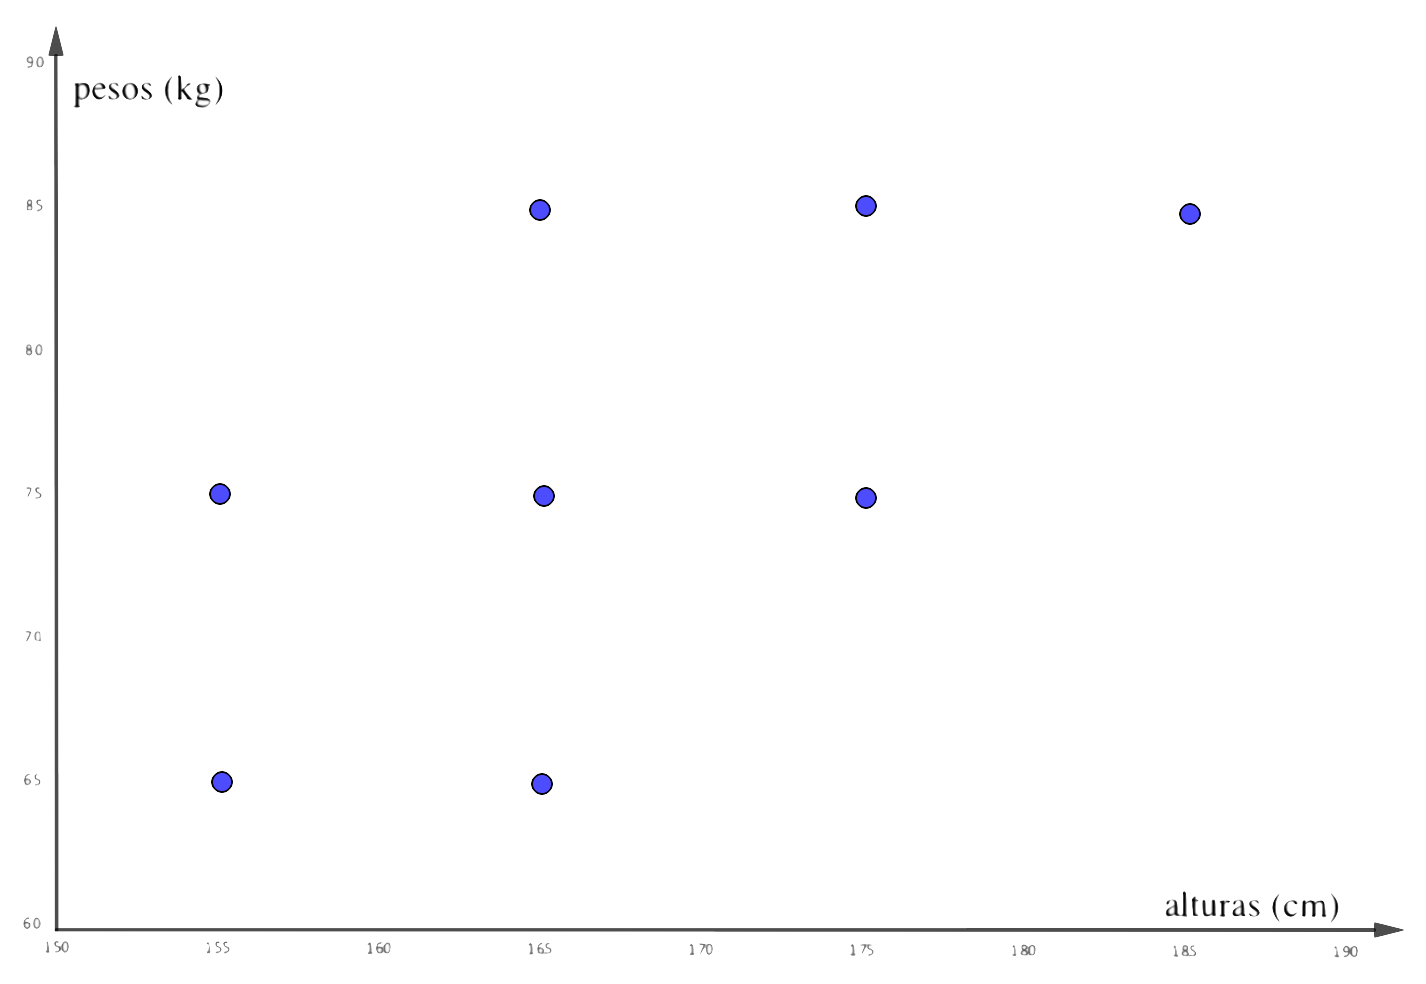
\includegraphics[width=0.75\textwidth]{imagenes/imagenes03/T03IM01.png}
	\end{figure}

Si cada par de variables tiene su propia frecuencia tenemos dos soluciones: o bien dibujamos tantos puntos próximos entre sí como indique la frecuencia absoluta, o bien dibujamos para cada pareja de valores círculos de área proporcional a la frecuencia absoluta de los mismos ($A=\pi r^2 \propto n_{ij} \to r \propto \sqrt{n_{ij}};\ $ --- \textcolor{gris}{$\propto$ es el símbolo de proporcionalidad}).

\begin{figure}[H]
			\centering
			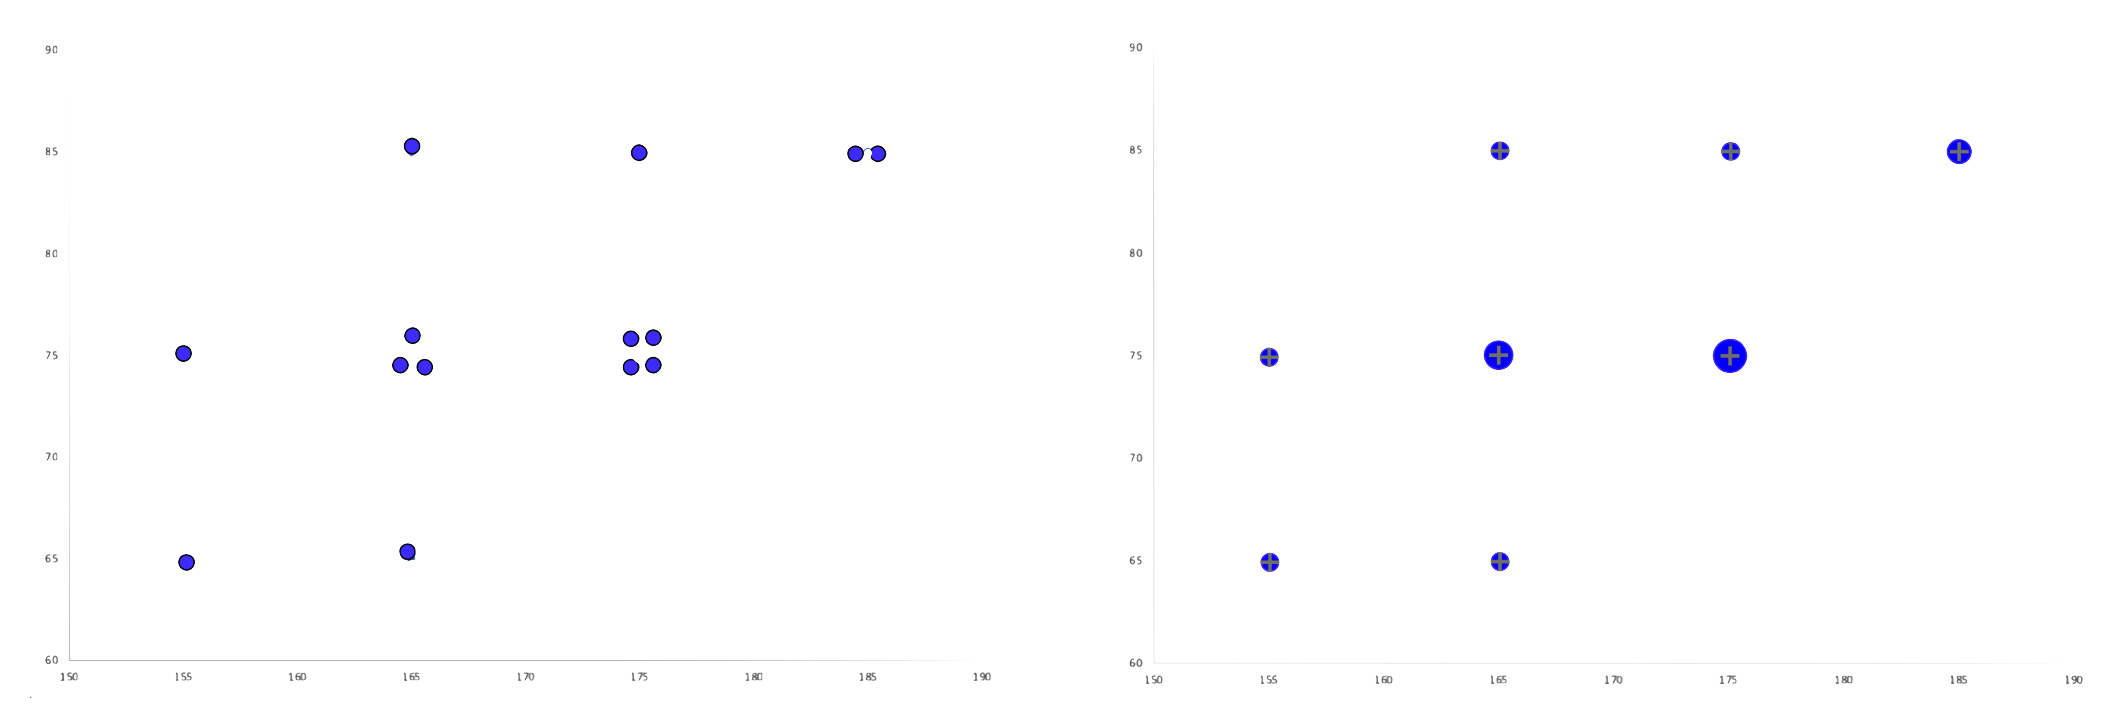
\includegraphics[width=0.95\textwidth]{imagenes/imagenes03/T03IM02.png}
	\end{figure}

Otra posibilidad es usar el \emph{prismograma}, es una representación 3D, en la base se representa la variable X-Y, $(x_i,y_i)$, y como altura la frecuencia absoluta de cada valor de la variable bidimensional, $n_{ij}$, formando una barra o un prisma (todos de la misma base).

	\begin{figure}[H]
			\centering
			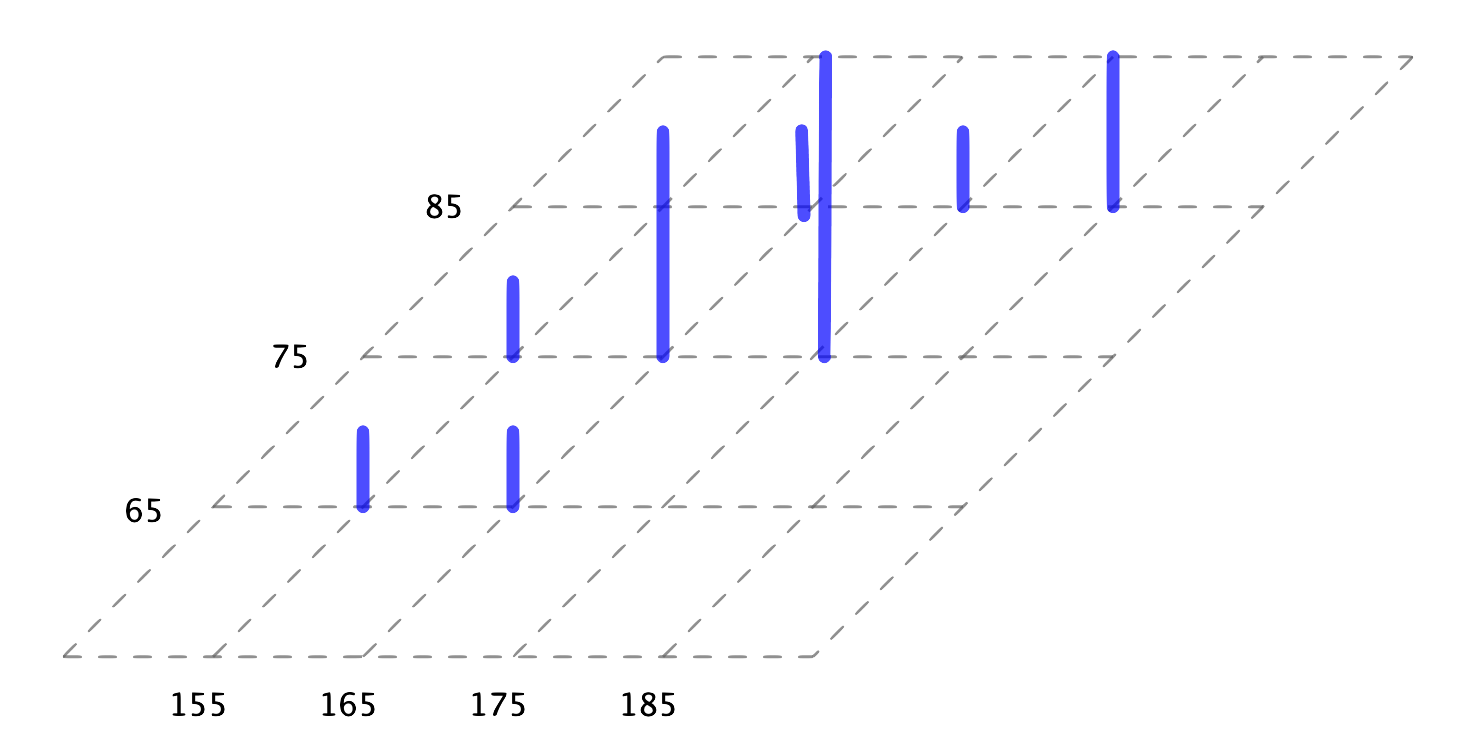
\includegraphics[width=0.65\textwidth]{imagenes/imagenes03/T03IM03.png}
	\end{figure}

\end{definition}




\subsection{Parámetros de las distribuciones bidimensionales}


\begin{definition}
. Considerando las variables X e Y por separado, como variables unidimensionales, tenemos las \textbf{variables marginales}.

\vspace{2mm} \begin{small} En la tabla de doble entrada, la última fila y la última columna son las frecuencias absolutas de las variables marginales. En las tablas de simple entrada, para trabajar con las variables marginales, basta con obviar cualquiera de ellas dos para considerar la otra. \end{small}

\vspace{2mm} Para cada una de las variables \textbf{marginales} podemos calcular su \textbf{\emph{valor medio}}, su \textbf{\emph{varianza}} y su \textbf{\emph{desviación típica}}. Así, tendremos:

$$X\ \to \ \bar x;\quad s^2_x;\quad s_x\ ;\qquad \qquad \qquad
Y\ \to \ \bar y;\quad s^2_y;\quad s_y$$
\end{definition}

\begin{definition}
.	\textbf{Covarianza}.  Se define la \emph{covarianza} de una distribución bidimensional, $\boldsymbol{s_{xy}}$, a la media aritmética de los productos de las desviaciones da cada uno de los valores de la variable bidimensional respecto a sus respectivos valores medios:

$$\boldsymbol{s_{xy}} \ = \ 
\dfrac{ \displaystyle \sum_{i=1}^m \ \sum_{j=1}^r \ (x_i-\bar x)\cdot (y_i-\bar y) \cdot n_{ij}}{N} \ = \ 
\dfrac{\displaystyle \sum_{i=1}^m \ \sum_{j=1}^r \ x_i \ y_i \  n_{ij}}{N} \ - \ \bar x \cdot \bar y$$
\end{definition}

\textcolor{gris}{La última igualdad es fácilmente demostrable sin más que desarrollar el producto que aparece en la definición de covarianza.}

\begin{destacado}
La covarianza nos proporciona información acerca del grado de dependencia existente entre las variables. El signo de la covarianza nos proporciona información sobre el sentido de esa dependencia: 

--- Si la covarianza es positiva las dos variables varían en el mismo sentido; si aumenta una, aumentará la otra ($X\uparrow \Rightarrow Y\uparrow$).

--- Si la covarianza es negativa las dos variables varían en sentido contrario; si aumenta una, disminuirá la otra ($X\uparrow \Rightarrow Y\downarrow$).
\end{destacado}

\begin{example}
.	Vamos a realizar, a mano, todos los cálculos para la distribución de los ejemplos anteriores.	 Como dijimos  en el tema de estadística, también para estadística bidimensional, con el sw. apropiado o calculadora adecuada, todos estos cálculos se obtienen muy rápidamente. Usamos el método manual para reforzar el significado de los parámetros.

\begin{table}[H]
\centering
\begin{tabular}{c|c|c|c|c}
$\boldsymbol{\downarrow X \ \ / \ \ Y \rightarrow}$ & \textbf{{[}60,70{[}$\to 65$} & \textbf{{[}70,80{[}$\to 75$} & \textbf{{[}80,90{[}$\to 85$} & \textbf{$n_{x_i}$} \\ \hline
\textbf{{[}150,160{[}$\to 155$} & 1 & 1 & 0 & 2 \\ \hline
\textbf{{[}160,170{[}$\to 165$} & 1 & 3 & 1 & 5 \\ \hline
\textbf{{[}170,180{[}$\to 175$} & 0 & 4 & 1 & 5 \\ \hline
\textbf{{[}180,190{[}$\to 185$} & 0 & 0 & 2 & 2 \\ \hline
\textbf{$n_{y_j}$} & 2 & 8 & 4 & \textbf{14}
\end{tabular}
\end{table}

	\begin{figure}[H]
			\centering
			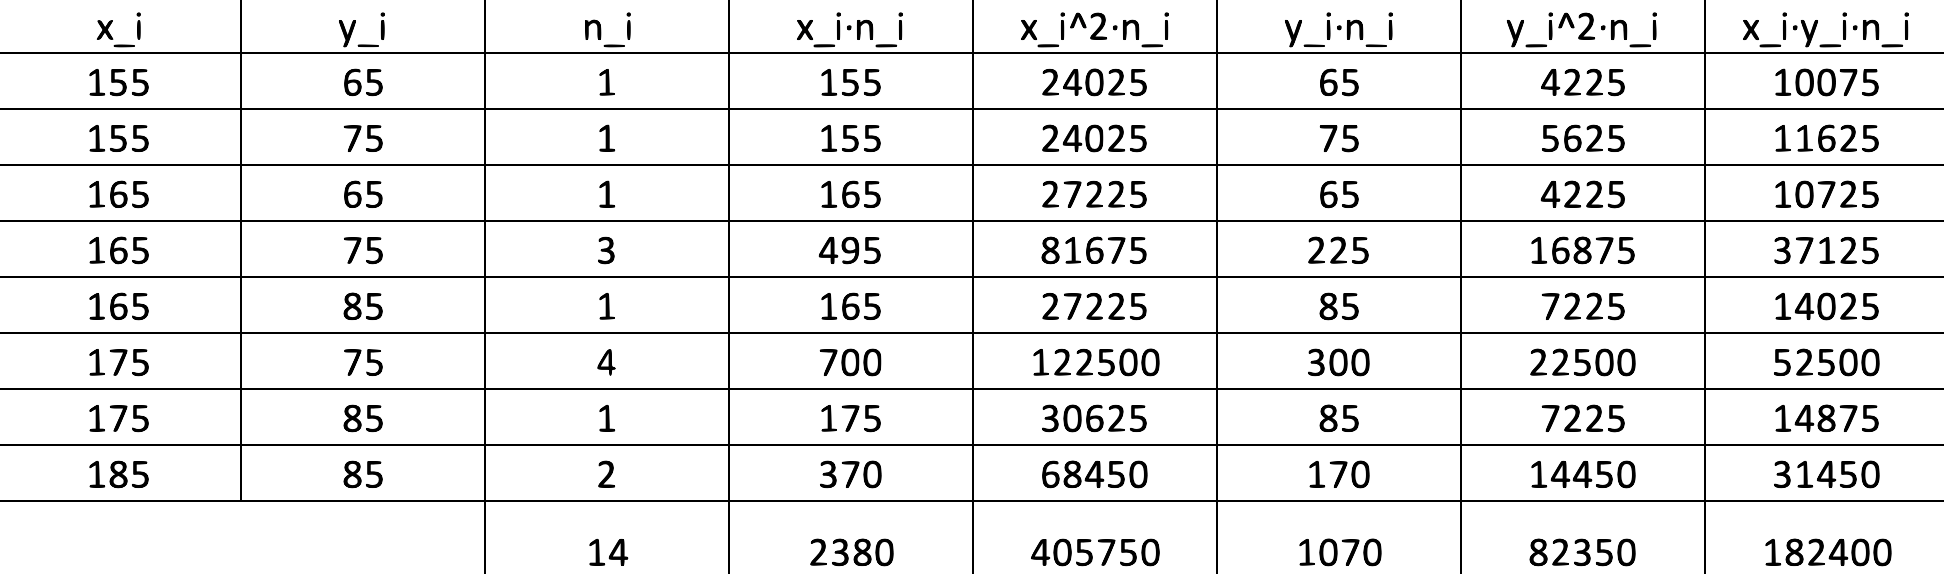
\includegraphics[width=0.95\textwidth]{imagenes/imagenes03/T03IM04.png}
	\end{figure}

\begin{multicols}{2}
$\bar x=\dfrac{2380}{14}=170$

$\quad$

$s_x=\sqrt{\dfrac{405750}{14}-170^2}=9.06$

$\bar y=\dfrac{1070}{14}=76.43$	

$\quad$

$s_y=\sqrt{\dfrac{82350}{14}-76.43^2}=6.37$
\end{multicols}
$$s_{xy}=\dfrac{182400}{14}-170\cdot 76.43=35.47$$

\end{example}


\section{Dependencia o Correlación}


En cursos de Análisis Matemático se estudian relaciones \emph{determinísticas}, si dos variables x e y están relacionadas de esa manera, sabiendo el valor de x, podemos conocer exactamente el valor de y.

En muchas aplicaciones encontramos variables que parecen estar relacionadas, aunque no de manera determinística. Esto significa que, saber el valor de una variable (la variable explicativa) no nos permite conocer exactamente el valor de la otra (la variable respuesta), ya que  ésta puede considerarse una variable aleatoria. Por ejemplo, sean `x' la edad de un niño e `y' su talla, sabemos que la talla depende de la edad, pero también depende de muchas otras condiciones; para una determinada edad, la talla puede considerarse como una variable aleatoria. Cuando ocurre esto decimos que las variables están \textbf{correlacionadas}, son estadísticamente dependientes.

\begin{definition}
.	Entre dos variables estadísticas existe \textbf{dependencia estadística o \emph{correlación}} cuando los valores que toma una de ellas están relacionados con los valores que toma la otra, pero no de manera exacta.	

La relación existente entre dos variables queda reflejada en los diagramas de dispersión o nubes de puntos de la distribución bidimensional.

--- Si los puntos de la nube se sitúan sobre una recta o una curva cuya expresión matemática podemos determinar, hablaremos de dependencia funcional entre las variables X e Y.

--- Si los puntos de la nube se agrupan en torno a una posible recta, o curva, no muy definida pero reconocible, hablaremos de dependencia estadística o correlación entre las variables X e Y.

--- Si los puntos de la nube no se agrupan en torno a ninguna curva, están completamente en desorden, hablaremos de independencia entre las variables X e Y.

	\begin{figure}[H]
			\centering
			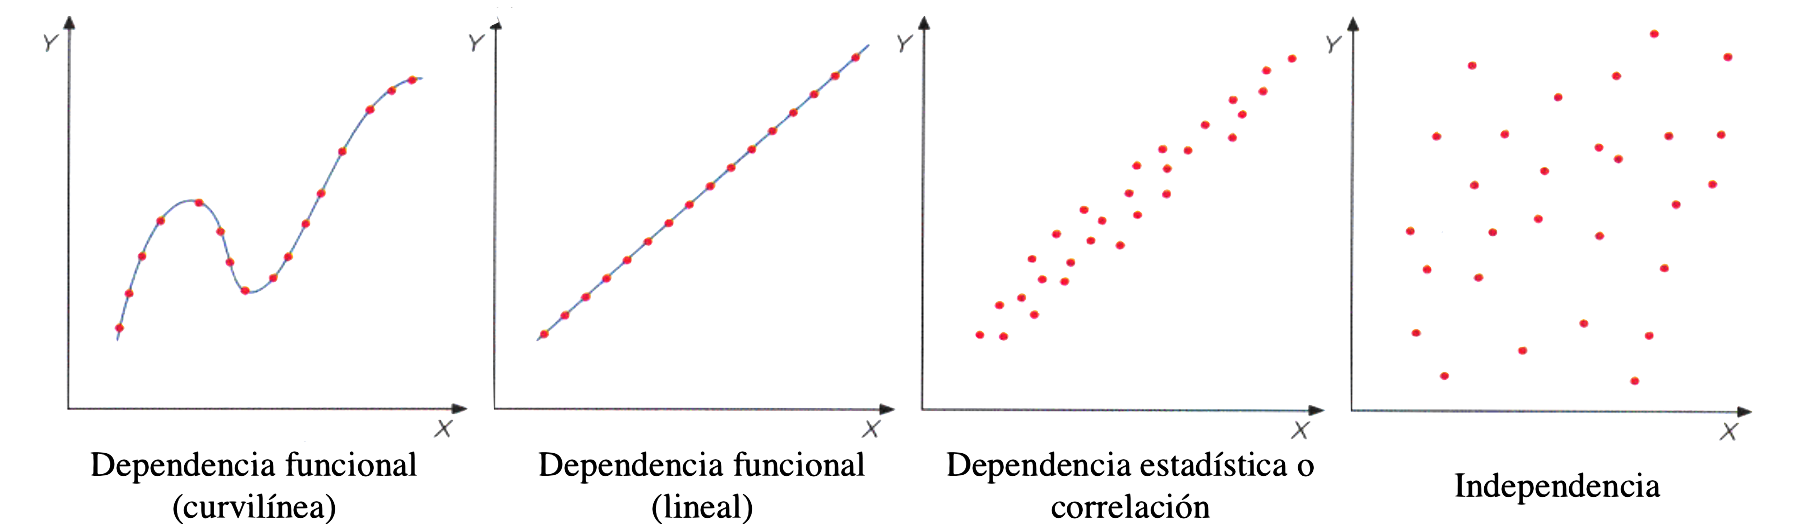
\includegraphics[width=0.95\textwidth]{imagenes/imagenes03/T03IM06.png}
			\caption*{\scriptsize{https://yoquieroaprobar.es/\_pdf/04140.pdf}}
	\end{figure}
	

\end{definition}

\section{Correlación lineal}

El caso más simple que estudiaremos en este capítulo, es el modelo de \textbf{regresión lineal}.

 El \textbf{coeficiente de correlación lineal de Pearson}, es un número \emph{adimensional} que sire para medir, de forma cuantitativa, la dependencia lineal de las variables X e Y.

\begin{definition}
.	El \textbf{coeficiente de correlación lineal} de Pearson mide una tendencia lineal entre dos variables numéricas.

\vspace{4mm} Es el método de correlación más utilizado y se necesita que:

\begin{itemize}
\item la tendencia debe ser de tipo lineal.
\item no existan valores atípicos (outliers).
\item las variables deben ser cuantitativas, si  son cualitaivas no podremos aplicar la correlación de Pearson.
\item debe haber suficientes datos (algunos autores recomiendan tener más de 30 puntos u observaciones).
\end{itemize}
Es de gran ayuda, para observar la tendencia lineal, el disponer del diagrama de dispersión o nube de puntos correspondiente.

El \textbf{coeficiente de correlación lineal}, $\boldsymbol{r}$, se define como:

$$\boxed{\ \boldsymbol{ r\ = \ \dfrac {s_{xy}}{s_x \cdot s_y} }  \ }$$

\vspace{3mm} %*****************************
\begin{itemize}
\item $\boldsymbol{-1 \ \le \ r \ \le 1}	$
\item Si $\ |r|=1 \to $ relación funcional
\item Si $\ r=0 \to $ variables incorreladas, no hay dependencia entre ellas.
\item Si $\ r>0\to $ correlación positiva o directa; Si $\ r<0\to $ correlación negativa o inversa.
\item Si $\ |r|\approx 1 \to $ correlación muy fuerte.
\end{itemize}

\vspace{5mm} %*****************************
	\begin{figure}[H]
			\centering
			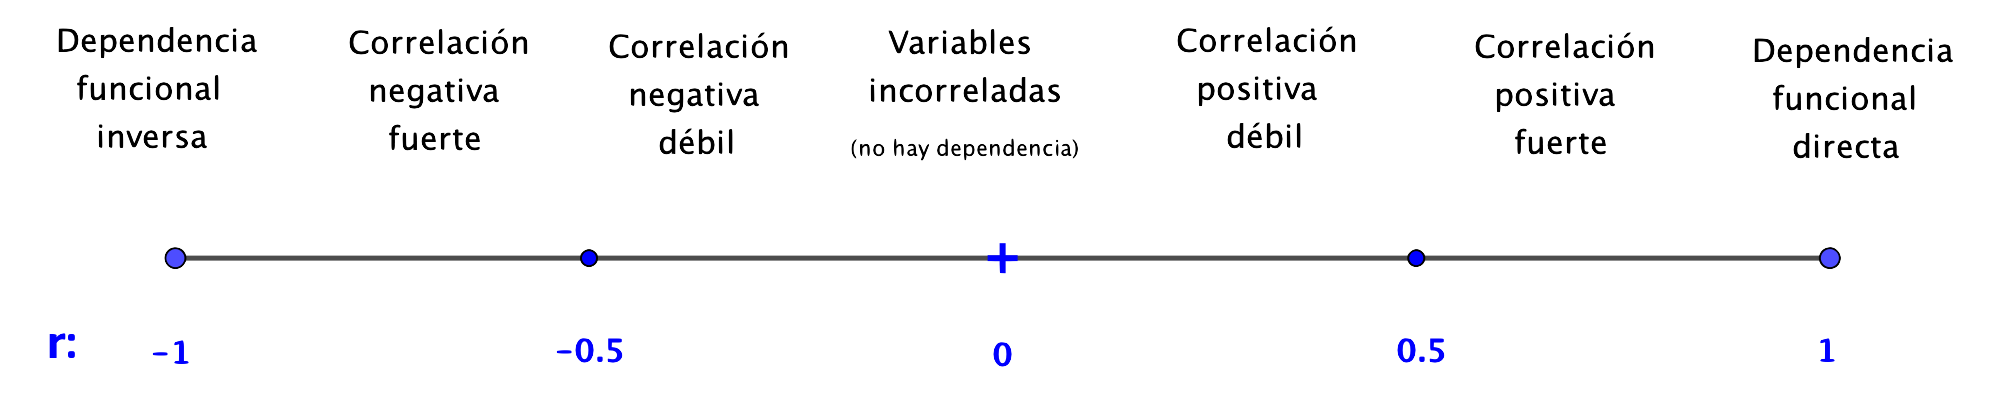
\includegraphics[width=0.95\textwidth]{imagenes/imagenes03/T03IM07.png}	
		\end{figure}
		

\vspace{5mm} \underline{Coeficiente de correlación y diagrama de dispersión:}

\vspace{5mm} %*****************************
		\begin{figure}[H]
			\centering
			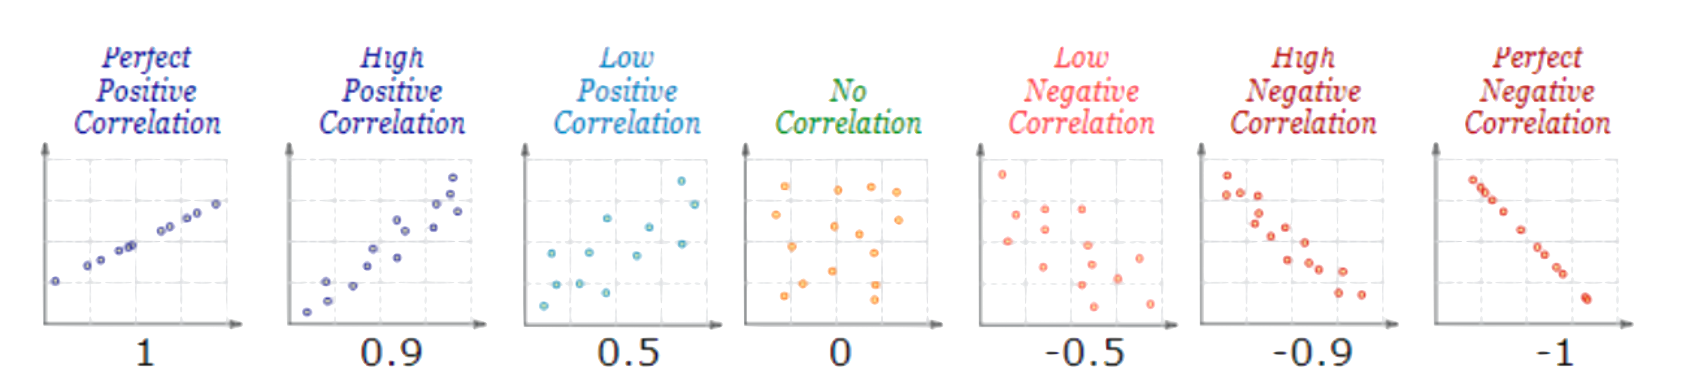
\includegraphics[width=0.95\textwidth]{imagenes/imagenes03/T03IM05.png}
			\caption*{\scriptsize{imagen de https://www.maximaformacion.es/blog-dat/que-es-la-correlacion-estadistica-y-como-interpretarla/}}
	\end{figure}
\end{definition}

\vspace{10mm} %*****************************
\begin{multicols}{2}
\underline{Observación} 

No es suficiente el cálculo del coeficiente de correlación para negar la dependencia entre dos variables. Puede haber casos en que $r=0$ y sin embargo existir un tipo de dependencia (aunque no lineal) entre las variables.

	\begin{figure}[H]
			\centering
			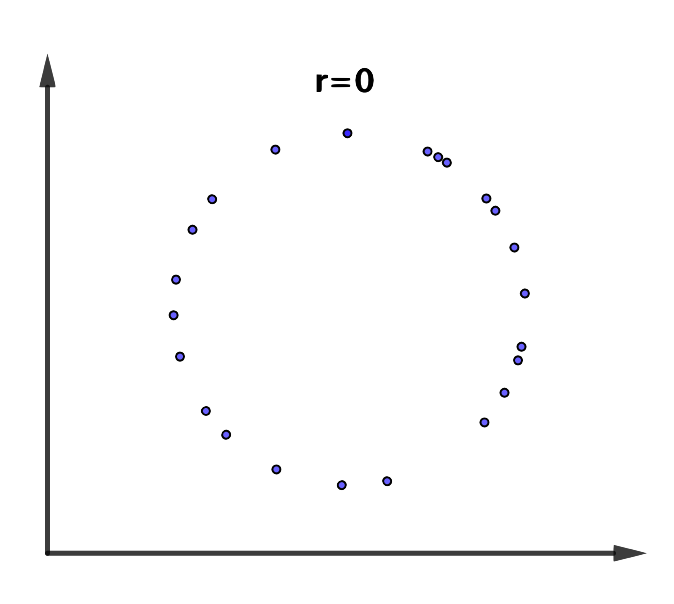
\includegraphics[width=0.3\textwidth]{imagenes/imagenes03/T03IM10.png}
	\end{figure}
\end{multicols}

	
\section{Regresión lineal}

\begin{theorem}
.	Dada la variable estadística bidimensional $(x_i, \ y_i; \ n_{ij})$ \textcolor{gris}{($(x_i,\ y_i,\ n_i) $, en tablas de entrada simple))}, si el diagrama de dispersión indica una dependencia lineal y el coeficiente de correlación lineal confirma una correlación fuerte, la \emph{recta} $y=a+bx$ que mejor se ajusta a la nube de puntos es la \textbf{recta de regresión}, de ecuación:

$$ \boxed{\ \  \boldsymbol{ y-\bar y \ =\  \dfrac {s_{xy}}{s_x^2}\  (\ x-\bar x\ ) }\ \  }$$
\end{theorem}

\begin{proof}\textcolor{white}{.}

	Para encontrar esta expresión usaremos el \textbf{método de los mínimos cuadrados}.

\begin{multicols}{2}
$\quad$

% Please add the following required packages to your document preamble:
% \usepackage{multirow}
\begin{table}[H]
\centering
\begin{tabular}{c|c|c|c}
\multirow{2}{*}{\begin{tabular}[c]{@{}c@{}}Variable\\ estad. 2dim\end{tabular}} & $\boldsymbol {x_i}$ & $\boldsymbol {y_i}$ & $\boldsymbol {n_i}$ \\ \cline{2-4} 
 & $\cdots$ & $\cdots$ & $\cdots$
\end{tabular}
\end{table}


$$ y\ =\ a\ +\ bx$$

$$y_{ri}=a+bx_i;\qquad d_i=y_i-y_{ri}$$

$\quad$
	\begin{figure}[H]
			\centering
			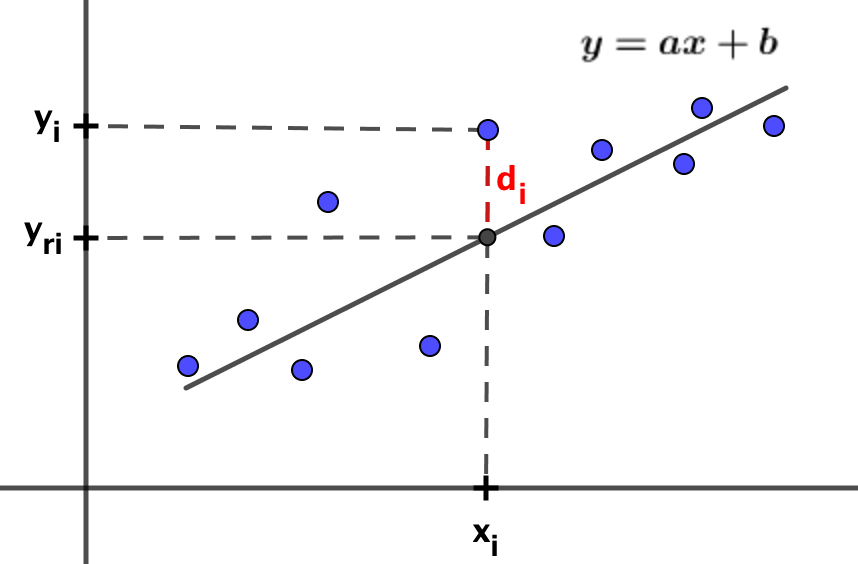
\includegraphics[width=0.5\textwidth]{imagenes/imagenes03/T03IM08.png}
	\end{figure}
\end{multicols}

El \emph{método de los mínimos cuadrados} consiste en encontrar los coeficientes $\boldsymbol{a}$ y $\boldsymbol{b}$ de la recta $\boldsymbol{y=a+bx}$ tal que la suma de los cuadrados de las distancias, $D$, da cada punto a la recta sea \textbf{mínima}. Una vez encontrada esta recta, recibe el nombre de \textbf{recta de regresión}.


$D=d_1^2+d_2^2+\cdots +d_N^2=\displaystyle  \sum_{i=1}^N \ d_i^2 = \sum_{i=1}^N \ [\ y_i-(a+bx_i)\ ]^2$
Puesto que $D=D(a,b)$, por análisi matemático sabemos que el mínimo ha de verificar que las derivadas de $D$ sean cero: $\displaystyle \pdv{D}{a}=\pdv{D}{b}=0$

\vspace{3mm} $\begin{cases}
\ \ \displaystyle \pdv{D}{a}\ =\ -2 \sum_{i=1}^N\ [ \  y_i-(a+bx_i)  \ ]	 \ = \ 0
\\
\ \ \displaystyle \pdv{D}{b}\ =\ -2 \sum_{i=1}^N\ [ \  y_i-(a+bx_i)  \ ]\cdot x_i	 \ = \ 0
\end{cases}$

\vspace{3mm} $\to \ \begin{cases}
\ \ \displaystyle   \sum_{i=1}^N\ y_i - Na - b\sum_{i=1}^N \ x_i \ = \ 0
\\
\ \ \displaystyle   \sum_{i=1}^N\   y_i\cdot x_i - a\sum_{i=1}^N\ x_i - b\sum_{i=1}^N\ x_i^2	 \ = \ 0
\end{cases}$


\vspace{3mm} Dividiendo por $N$, 
$\quad \begin{cases}
\ \ \bar y - a - b\bar x=0 
\\ 
\ \  \dfrac{\displaystyle \sum_{i=1}^N\ x_i\ y_i}{N} - a\bar x - b \dfrac {\displaystyle \sum_{i=1}^N\ x_i^2}{N}
\end{cases} \ \to \ 
\begin{cases}
\ \ a=\bar y - b \bar x \\ 
\\ s_{xy}+\bar x\ \bar y-a\bar x-b(s_x^2+{\bar x}^2) 	
\end{cases}$

\vspace{3mm} Resolviendo el sistema, $\ \ \begin{cases}
\ \ a=\bar y - \dfrac{s_{xy}}{s_x^2} \ \bar x \\ \ \ b=\dfrac{x_{xy}}{s_x^2}	\end{cases}$, con lo que la recta de regresión buscada es:

$\subrayado{\  \boxed { \ \boldsymbol{ y-\bar y \ = \ \dfrac{s_{xy}}{s_x^2}\ (x-\bar x) } \ } \ } \quad $ \textbf{Recta de regresión de Y sobre X}. 

A la pendiente,  $\boldsymbol{ \ \dfrac{s_{xy}}{s_x^2}\ = \ m_{YX} \  }$, se le llama \textbf{coeficiente de regresión de Y sobre X}. Y es la variable dependiente (explicada) y X es la variable independiente (explicativa). 

La \emph{recta de regresión de Y sobre X} sirve para \emph{hacer predicciones sobre la Y sabida la X}. Si lo que deseamos es \emph{hacer predicciones sobre la X sabida la Y}, necesitaremos la \emph{recta de regresión de X sobre Y}, que se obtiene de modo análogo a la anterior pero considerando ahora la X como variable dependiente (explicada) y la Y como variable independiente (explicativa). Es decir, intercambiando los papeles de X e Y:

$\subrayado{\  \boxed { \ \boldsymbol{ x-\bar x \ = \ \dfrac{s_{xy}}{s_y^2}\ (y-\bar y) } \ } \ } \quad $ \textbf{Recta de regresión de X sobre Y}. 

A la pendiente,  $\boldsymbol{ \ \dfrac{s_{xy}}{s_y^2}\ = \ m_{XY} \  }$, se le llama \textbf{coeficiente de regresión de X sobre Y}. X es la variable dependiente (explicada) e Y es la variable independiente (explicativa).

\end{proof}

\begin{definition}
.	Hay pues dos rectas de regresión:

$$\subrayado{\  \boxed { \ \boldsymbol{ y-\bar y \ = \ \dfrac{s_{xy}}{s_x^2}\ (x-\bar x) } \ } \ } \quad  \textbf{Recta de regresión de Y sobre X}.$$ 

$$\subrayado{\  \boxed { \ \boldsymbol{ x-\bar x \ = \ \dfrac{s_{xy}}{s_y^2}\ (y-\bar y) } \ } \ } \quad  \textbf{Recta de regresión de X sobre Y}. $$

La primera sirve para hacer predicciones sobre los valores de Y mientas que la segunda se usa para hacer predicciones sobre la X.	
\end{definition}

\begin{theorem}
.	$$ r\ = \ \dfrac{s_{xy}}{s_x\cdot s_y} \ = \ \pm \sqrt{m_{YX}\cdot m_{XY}}	$$

El signo de $r$ coincide con el de $s_{xy}$.
\end{theorem}

\vspace{-5mm} %***************************
\begin{proof}\textcolor{white}{.}

Evidente, $\ \dfrac{s_{xy}}{s_y^2}\ = \ m_{XY};\quad \dfrac{s_{xy}}{s_x^2}\ = \ m_{YX} $, por lo que	$\ m_{YX}\cdot m_{XY}=\dfrac{s_{xy}}{s_y^2}\  \dfrac{s_{xy}}{s_x^2}=r^2$
\end{proof}

\begin{theorem}
.	Propiedades de las dos rectas de regresión.

\begin{itemize}

\item Las dos rectas de cortan en el punto $(\bar x, \bar y)$, llamado \emph{centro de gravedad} de la nube de puntos (diagrama de dispersión).

\item Las pendientes de las dos rectas $m_{YX}$ y $m_{XY}$ tienen el mismo signo, que a su vez es igual al signo del coeficiente de correlación lineal $r$. Dicho signo lo dicta el de la covarianza $s_{xy}$.

\item En los casos en los que tenemos correlación perfecta (funcional), $r=\pm 1$, ( XY XY ), las dos rectas de regresión coinciden. De no ser así, forman un determinado ángulo que es mayor cuando menor es la correlación, siendo máximo ($90^o$) cuando las variables son incorreladas, $r=0$, en este caso las rectas son perpendiculares ($x=\bar x;\ y=\bar y$).

	\begin{figure}[H]
			\centering
			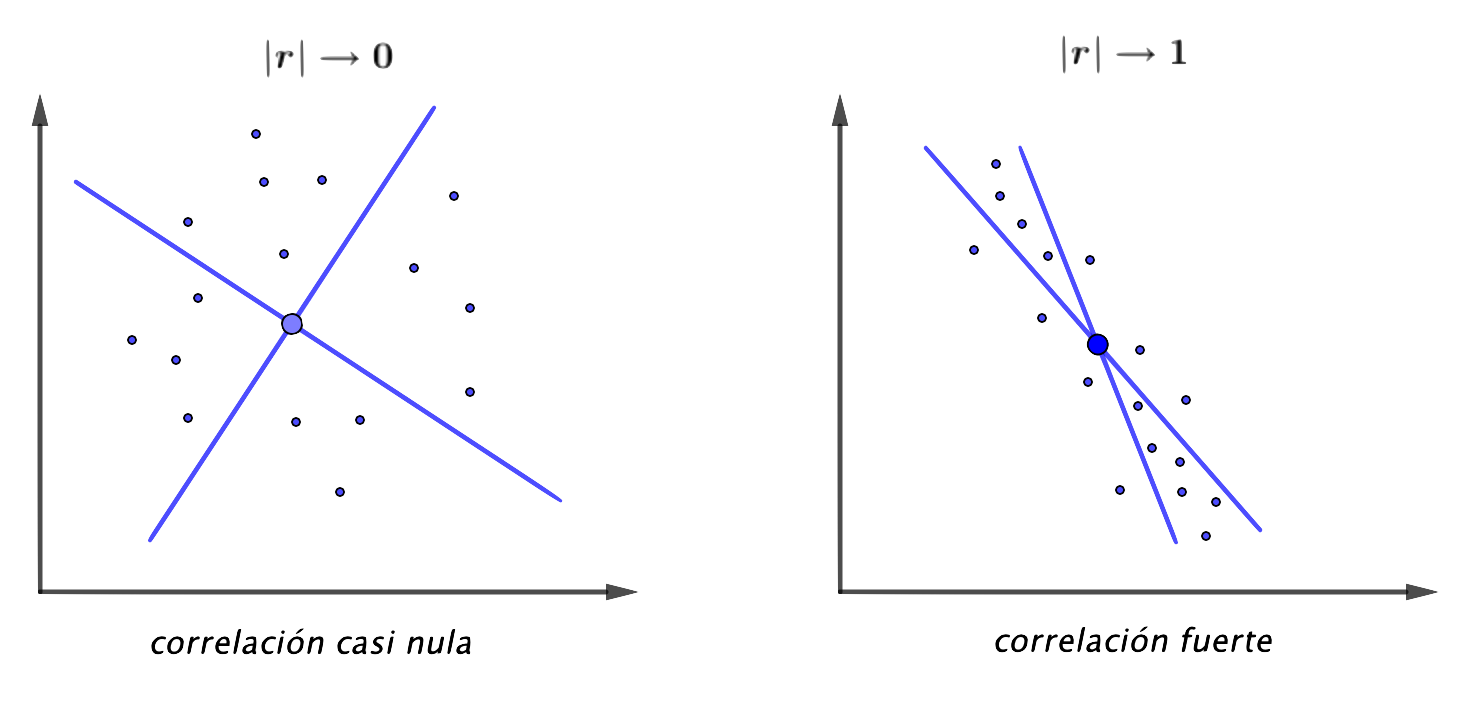
\includegraphics[width=0.6\textwidth]{imagenes/imagenes03/T03IM09.png}
	\end{figure}
\end{itemize}
\end{theorem}

\section{Coeficiente de determinación}

\textbf{\emph{El coeficiente de determinación mide la bondad del ajuste de la recta de regresión}}

\vspace{5mm} %****************************
\begin{definition}
	
El coeficiente de correlación lineal indica el grado de linealidad entre las dos variables, pero para analizar la bondad del ajuste de la recta de regresión se utiliza un parámetro nuevo llamado \textbf{coeficiente de determinación}, $\boldsymbol{ r^2 }$, indica el porcentaje de la variación de Y que puede ser explicada por X y, también, de la X respecto de la Y puesto que $r^2$ coincide coincide para las dos rectas de regresión:
$\ \ r^2 \ = \ \dfrac{s_{xy}^2}{s_x^2\cdot s_y^2} \ = \ m_{XY}\cdot m_{YX}$

Como $0 \le r^2 \le  1$, la interpretación de esta medida es similar a la de $r$:

\begin{itemize}
\item Si $r^2 = 0$, significa que no existe tal relación lineal entre las variables (puede existir otro tipo de relación o no haber ninguna entre las dos variables, incorreladas). No tendría sentido utilizar las rectas de regresión para analizar la influencia de X sobre Y, ni para predecir el valor de Y, dado X.

\item Si $r^2 = 1$, significa que el ajuste es perfecto (funcional). Las rectas pasan por todos los puntos de la nube, obviamente porque éstos están alineados y proporcionan toda la información sobre el comportamiento de Y en función de X, así como de X para Y,para la muestra considerada.

\item Si $0 < r^2 < 1$, habrá una determinada correlación lineal entre las variables, mayor cuanto más se aproxime a uno el coeficiente de determinación. Como $r^2$ , indica el \emph{porcentaje de la variación de Y que puede ser explicada por X} o al revés, un valor concreto de $r^2$ se puede interpretar en los siguientes términos: si $r^2 =0,92$, por ejemplo,  significa que las rectas obtenidas explican en un 92\% el comportamiento de una variable en función de la otra. El 8\% restante de la variación puede deberse al azar o a la influencia  de otras variables distintas.
\end{itemize}

\end{definition}


	

\vspace{15mm} %************************************
\begin{adjustwidth}{25pt}{25pt}
	\textcolor{gris}{\rule{70mm}{0.1mm}}
\vspace{5mm} %************************************
	\begin{destacado}
	Un coeficiente de determinación alto implica la relación lineal entre las variables es fuerte, pero eso no tiene por qué implicar que los cambios en una variable se expliquen por la otra variable. Así, si consideramos la variable (X,Y) en que X representa los ingresos mensuales de una muestra de 100 familias de una determinada ciudad e Y representa la asignación media asignada a sus hijos, el cambio brusco en los ingresos mensuales de una familia puede explicar un descenso de la asignación que dan a sus hijos, pero un descenso en la asignación a los hijos no explica el cambio en los ingresos de la familia (podría ser un castigo).
	
	Si existe una relación causal entre dos variables, la correlación por sí misma no nos dice nada sobre la dirección de la causalidad.
	\begin{flushright}
		\textit{\textbf{Correlación no implica causalidad.}}
	\end{flushright} 
	\end{destacado}
	\begin{flushright}
	\rule{70mm}{0.1mm}	
	\end{flushright}
\end{adjustwidth}
\vspace{1cm}

\subsection{Valoración de las predicciones. Interpolación y extrapolación}

\begin{definition}
	
La recta de regresión nos permite predecir valores de una variable a partir de los de la otra. No obstante, hay que tener siempre presente que existen las siguientes limitaciones:

\begin{itemize}
\item Las predicciones realizadas a partir de una recta de regresión no son fiables si entre X e Y no hay un alto grado de correlación lineal, es decir, si r no es, en valor absoluto, cercano a 1.
\item Las predicciones deben hacerse con valores próximos a los pares considerados. Las estimaciones obtenidas para valores próximos al centro de gravedad de la distribución son más fiables que las obtenidas para valores muy alejados de él. 
\item Los valores que están dentro del rango de la variable explicativa son interpolaciones; las que están fuera, extrapolaciones. Extrapolar siempre supone un riesgo añadido, la variable explicada puede tener una dependencia lineal con la variable explicativa en el rango de valores, pero no tenerlo o no ser lineal fuera de este rango.
\item La fiabilidad de una recta de regresión es mayor cuanto mayor sea el número de datos considerados para calcularla, N.	
\item Se considera buena la predicción si $r^2>75\%$ y muy buena a partir de $r^2>90\%$. Si $r^2<60\%$, las predicciones serán poco fiables.
\end{itemize}
\end{definition}


\vspace{1cm} %***************************************
	\begin{figure}[H]
			\centering
			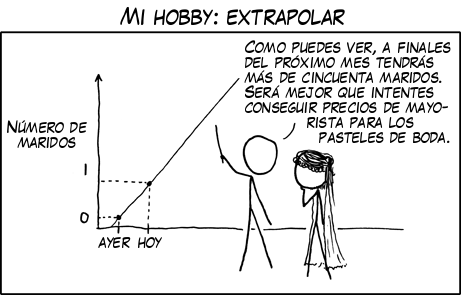
\includegraphics[width=0.6\textwidth]{imagenes/imagenes03/T03IM11.png}
	\end{figure}
\vspace{1cm} %***************************************

\begin{example}
.	Siguiendo con el ejemplo que nos ocupa en todo el tema:

	\begin{table}[H]
\centering
\begin{tabular}{c|c|c|c|c}
$\boldsymbol{\downarrow Y \ \ / \ \ X \rightarrow}$ & \textbf{{[}60,70{[}$\to 65$} & \textbf{{[}70,80{[}$\to 75$} & \textbf{{[}80,90{[}$\to 85$} & \textbf{$n_{x_i}$} \\ \hline
\textbf{{[}150,160{[}$\to 155$} & 1 & 1 & 0 & 2 \\ \hline
\textbf{{[}160,170{[}$\to 165$} & 1 & 3 & 1 & 5 \\ \hline
\textbf{{[}170,180{[}$\to 175$} & 0 & 4 & 1 & 5 \\ \hline
\textbf{{[}180,190{[}$\to 185$} & 0 & 0 & 2 & 2 \\ \hline
\textbf{$n_{y_j}$} & 2 & 8 & 4 & \textbf{14}
\end{tabular}
\end{table}


	\begin{figure}[H]
			\centering
			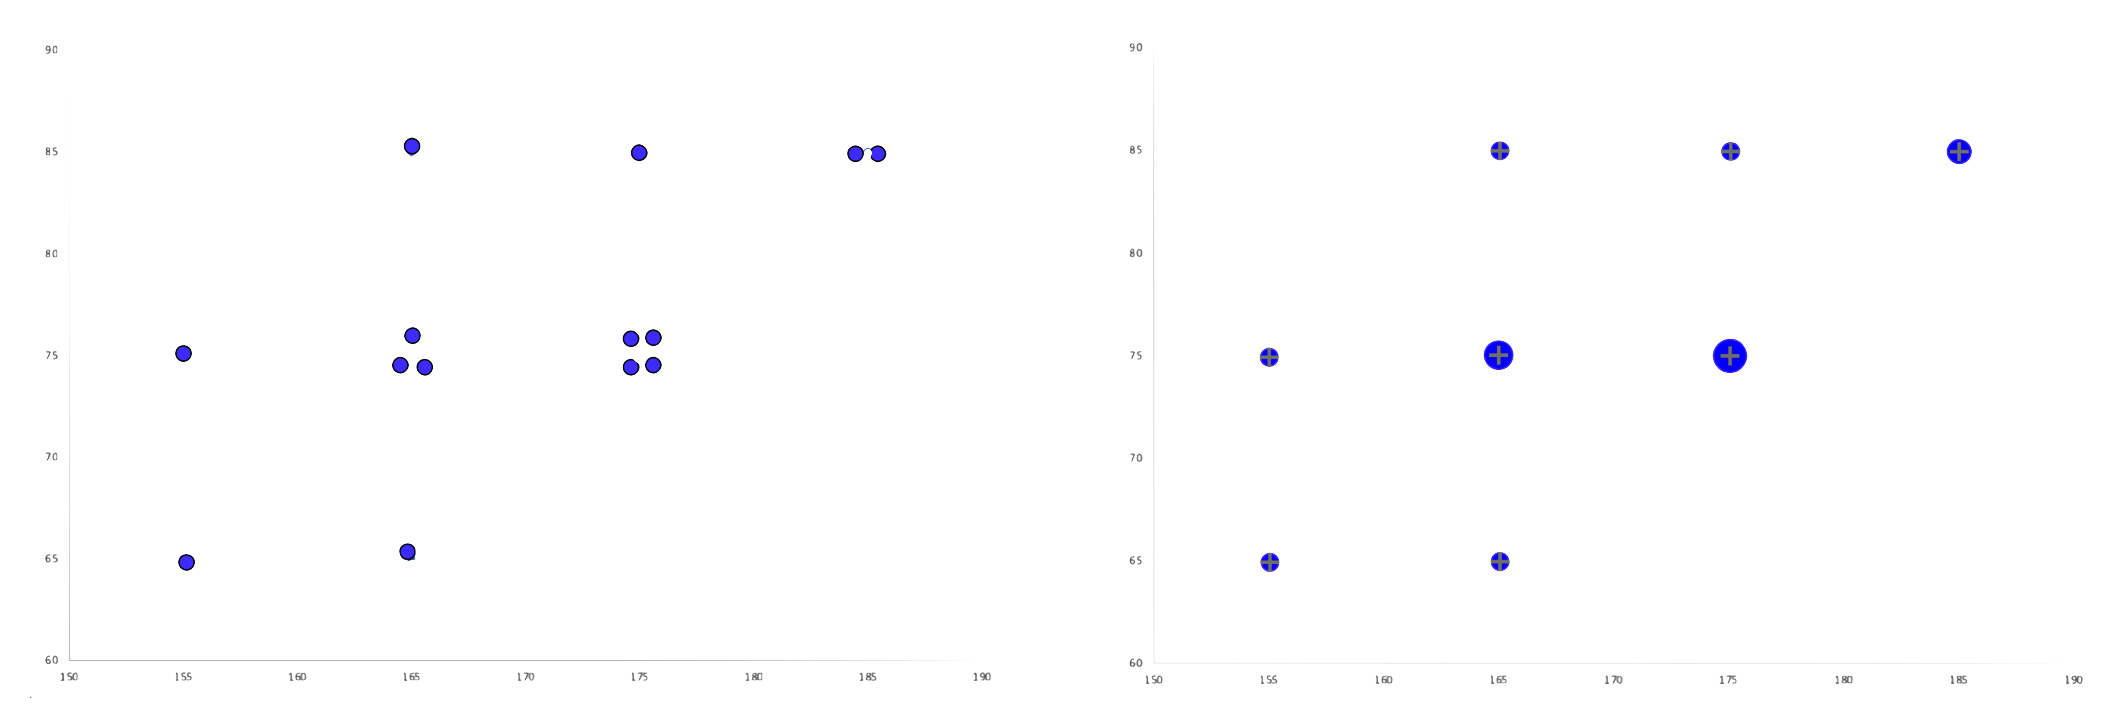
\includegraphics[width=0.95\textwidth]{imagenes/imagenes03/T03IM02.png}
	\end{figure}

$\qquad \bar x=\dfrac{2380}{14}=170;$$\quad$$s_x=\sqrt{\dfrac{405750}{14}-170^2}=9.06$

$\qquad \bar y=\dfrac{1070}{14}=76.43;$$\quad$$s_y=\sqrt{\dfrac{82350}{14}-76.43^2}=6.37$

$\qquad s_{xy}=\dfrac{182400}{14}-170\cdot 76.43=35.47$

\textcolor{green}{\rule{100mm}{0.1mm}}
	
\vspace{3mm} %**********************
Calcula el coeficiente de correlación lineal y el coeficiente de determinación. ?`Cómo es la dependencia de estas variables?

?`Cuál es el valor que debería tener la variable Y para un valor de X=77 Kg? ?Qué debería valer ya X si la Y=210 cm? ?`Cómo de fiables son estas predicciones?

\vspace{-3mm} \begin{center}\textcolor{green}{\rule{100mm}{0.1mm}}\end{center}

Ala vista del diagrama de dispersión, intuimos que va a haber una correlación positiva y débil. Calculemos el coeficiente de correlación:

\vspace{2mm} $r=\dfrac{s_{xy}}{s_x\cdot s_y}=\dfrac{35.47}{9.06\cdot 6.37}=0.61 \to$ correlación positiva y débil, no tiene demasiado sentido hacer predicciones.

\vspace{2mm} $r^2=0.61^2=0.38=38\%$, las predicciones explicarían el 38\% de los valors, el 63\% restante no.

\vspace{2mm} Aunque la correlación indica que las predicciones no serán fiables, vamos a hacerlas ya que las piden:

\vspace{2mm} --- Recta de regresión de X sobre Y:  $\ x-\bar x=\dfrac{s_{xy}}{s_y^2}(y-\bar y)$.

\vspace{2mm} $x-170=\dfrac{35.47}{6.37^2}(y-76.43) \ \to \ x=0.87y+103.19$

\vspace{2mm} Para un $y=77$ kg, obtenemos una $y=170.18$ cm.

\vspace{2mm} --- Recta de regresión de Y sobre X: $\ y-\bar y=\dfrac{}s_{xy}{x_x^2}(x-\bar x)$.

\vspace{2mm} $y-76.43=\dfrac{35.47}{9.06^2}(x-170) \ \to \ y=0.43x+2.97$

\vspace{2mm} Para una $x=210$ cm, obtenemos un $y=77$ Kg.

\vspace{2mm} Ya hemos advertido que las previsiones no son fiables dado que la correlación es débil (r=0.61). Aún así, la segunda previsión es mucho menos fiable que la primera pues se trata de una \emph{peligrosa} extrapolación, una altura de 210 cm está fuera de nuestro rango de valores, [150,190[.

En la siguiente figura mostramos las dos rectas de regresión así como las predicciones efectuadas. Obsérvese como la segunda predicción es una extrapolación.

\vspace{1cm} %***************************************
 
	\begin{figure}[H]
			\centering
			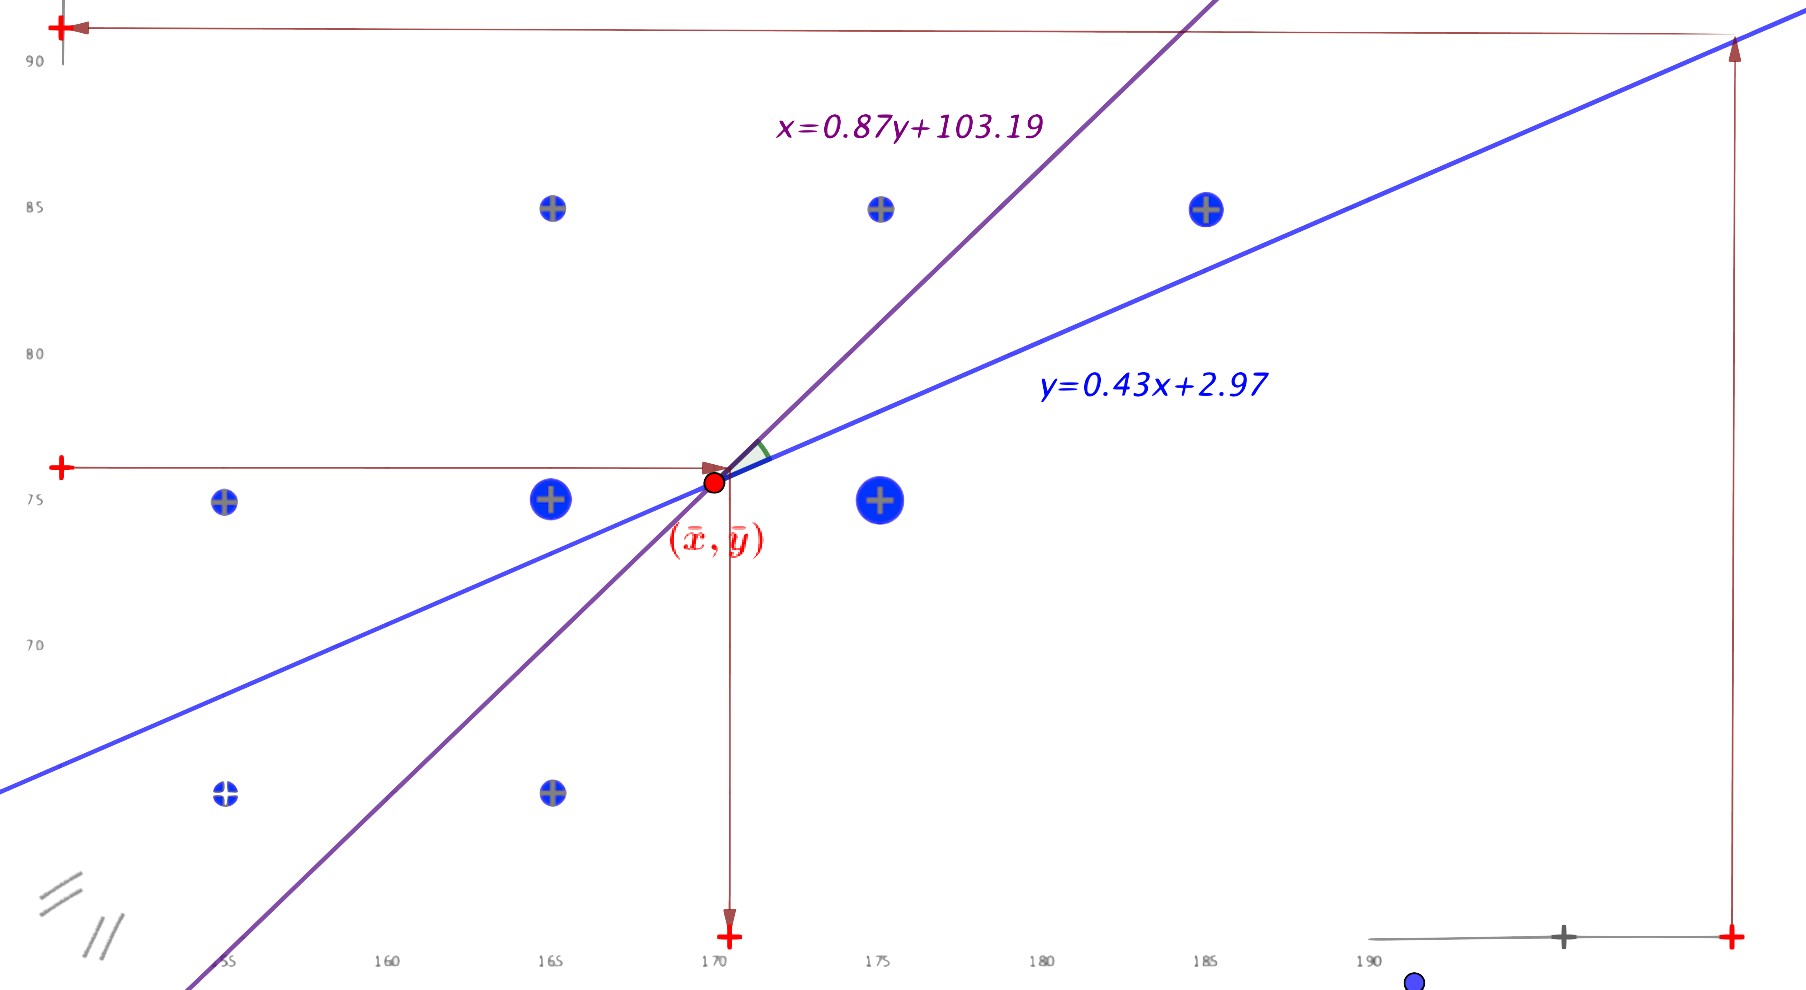
\includegraphics[width=0.75\textwidth]{imagenes/imagenes03/T03IM12.png}
	\end{figure}

\end{example}

\vspace{2cm} %***************************************

\begin{ejemplo}
\begin{ejre}
Las notas obtenidas en Matemáticas y Física por cinco alumnos son:

\begin{table}[H]
\centering
\begin{tabular}{l|rrrrr}
\textbf{Matemáticas (X)} & $\qquad 6$ &  $\ \ 4$ &  $\ \ 8$ &  $\ \ 5$ &  $\ \ 3.5$ \\ \hline
\textbf{Física (Y)} & $6.5$ & $4.5$ & $7$ & $5$ & $4$
\end{tabular}
\end{table}

\begin{adjustwidth}{20pt}{10pt}
\begin{enumerate}[a) ]
\item Dibujar el diagrama de dispersión y comentar si se espera o no que haya correlación lineal.
\item Calcular e interpretar los coeficientes de correlación lineal y de determinación.
\item Escribir las dos rectas de regresión.
\item Para una alumno de ese grupo que saque	 un 7.5 en matemáticas, ?`qué nota se espera que obtenga en física?
\item Si una alumno obtiene un 9 en física, ?cuál debería ser su nota en matemáticas?
\item Qué fiabilidad merecen las predicciones anteriores.
\end{enumerate}
\end{adjustwidth}
\vspace{5mm}

	\begin{figure}[H]
			\centering
			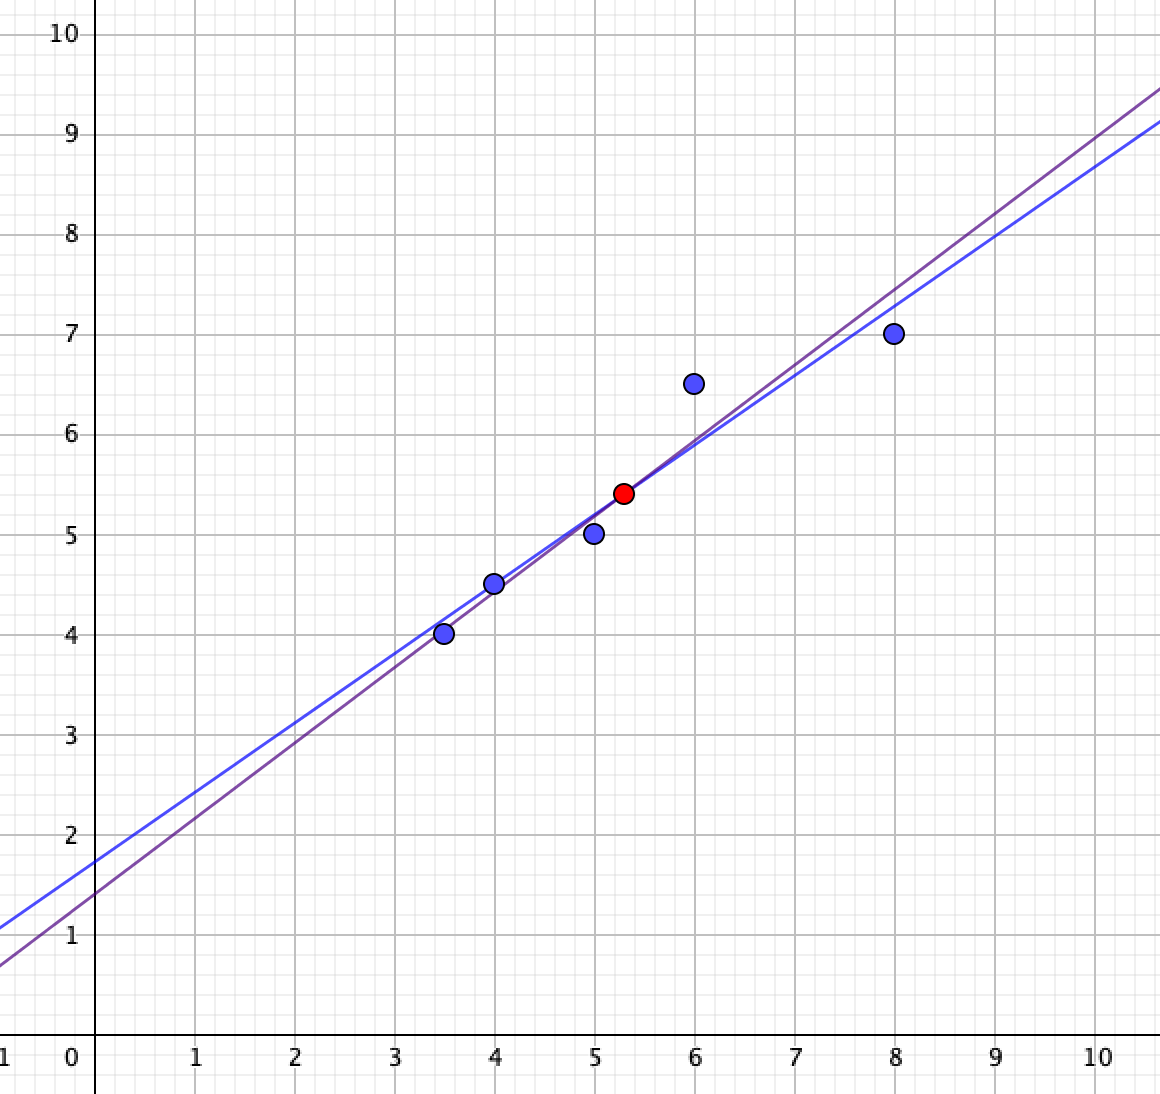
\includegraphics[width=0.75\textwidth]{imagenes/imagenes03/T03IM13.png}
	\end{figure}
--- a) A la vista de la nube de puntos, se espera una correlación positiva (o directa) y fuerte.

Se han incluído en el dibujo	 las dos rectas de regresión y en cdg centro de gravedad, $(\bar x, \bar y)$, de la nube de puntos (punto rojo).

--- b) y c). Cálculo de parámetros de la distribución bidimensional. Todos las frecuencias son 1, y N=5.

Con una sencilla hoja de cálculo obtenemos: $\Sigma x=26.5$, $\Sigma y=27$, $\Sigma x^2=153.25$, $\Sigma y^2=152.5$, $\Sigma x\cdot y=152$, por lo que:

$\bar x=5.3$; $s_x=1.6$; $\quad \bar y=5.4$; $s_y=1.16$; $\qquad s_{xy}=1.78$

De ahí: $\quad r=0.96; \qquad r^2=0.92=92\%$

Al ser $r=0.96$, la correlación es directa (positiva) y fuerte, habrá un alto grado de fiabilidad en las predicciones (ojo con las extrapolaciones). Por ser $r^2=92\%$, el $92\%$ de la nota de física es explicada por la de matemáticas y viceversa.

Las rectas de regresión son : $\quad y=0.695x+1.715; \qquad x=1.323y-1.843$

--- d), e) y f): predicciones.

$x=7.5 \to \textcolor{gris}{y=0.695x+1.715} \to y=6.93$

La predicción es altamente fiable dado el elevado coeficiente de correlación y el que se trata de una interpolación, $7.5\in [3.5,8]$

$y=9 \to \textcolor{gris}{x=1.323y-1.843} \to x=10.06$

La predicción es fiable por el elevado coeficiente de correlación pero arriesgada al tratarse de una extrapolación, $9\notin [4,7]$

\vspace{4mm} \textsf{De todos modos, el número de datos $N=5$ es muy pequeño para garantizar que las predicciones  tengan la fiabilidad necesaria.}
\end{ejre}	
\end{ejemplo}


\section{Recta de Tukey}

\begin{definition}
.	\vspace{2mm} La \textbf{recta de Tukey o recta mediana-mediana}	
permite ajustar una recta a una nube de puntos en algunos casos en los que el ajuste mínimo cuadrático produce resultados no muy buenos. La recta de Tukey o Mediana-Mediana es un método novedoso y práctico que puede venir a apoyar al que  hemos visto de  \emph{mínimos cuadrados} o \emph{recta de regresión}.

\vspace{2mm} La recta de Tukey\footnote{John Wilder Tukey (16 de junio de 1915 - 26 de julio de 2000). Estadístico estadounidense. Introdujo, además, los diagramas de cajas y bigotes.} es un método ingenioso que no requiere de un fundamento matemático demasiado abstracto en su tratamiento.

\vspace{2mm} Se utiliza cuando hay valores extraños (outliers) que, como sabemos, afectan mucho a las medias. Veremos como se calcula en el siguiente \textbf{ejemplo}.

\end{definition}

\begin{example}
.	Considera la siguiente distribución, dibuja la nube de puntos, la recta de regresión de Y sobre X y la recta de Tukey.

\begin{table}[H]
\centering
\begin{tabular}{l|rrrrrrrrrrrr}
\textbf{X} & 1 & 2 & 3 & 5 & 6 & 7 & 8 & \textcolor{red}{9} & 10 & 12 & 14 & \textcolor{red}{21} \\ \hline
\textbf{Y} & 9 & 11 & 13 & 13 & 15 & 14 & 16 & \textcolor{red}{1} & 16 & 14 & 19 & \textcolor{red}{2}
\end{tabular}
\end{table}
Hemos puesto en rojo los valores \emph{extraños}. Se ven a simple vista en el diagrama de dispersión.

	\begin{figure}[H]
			\centering
			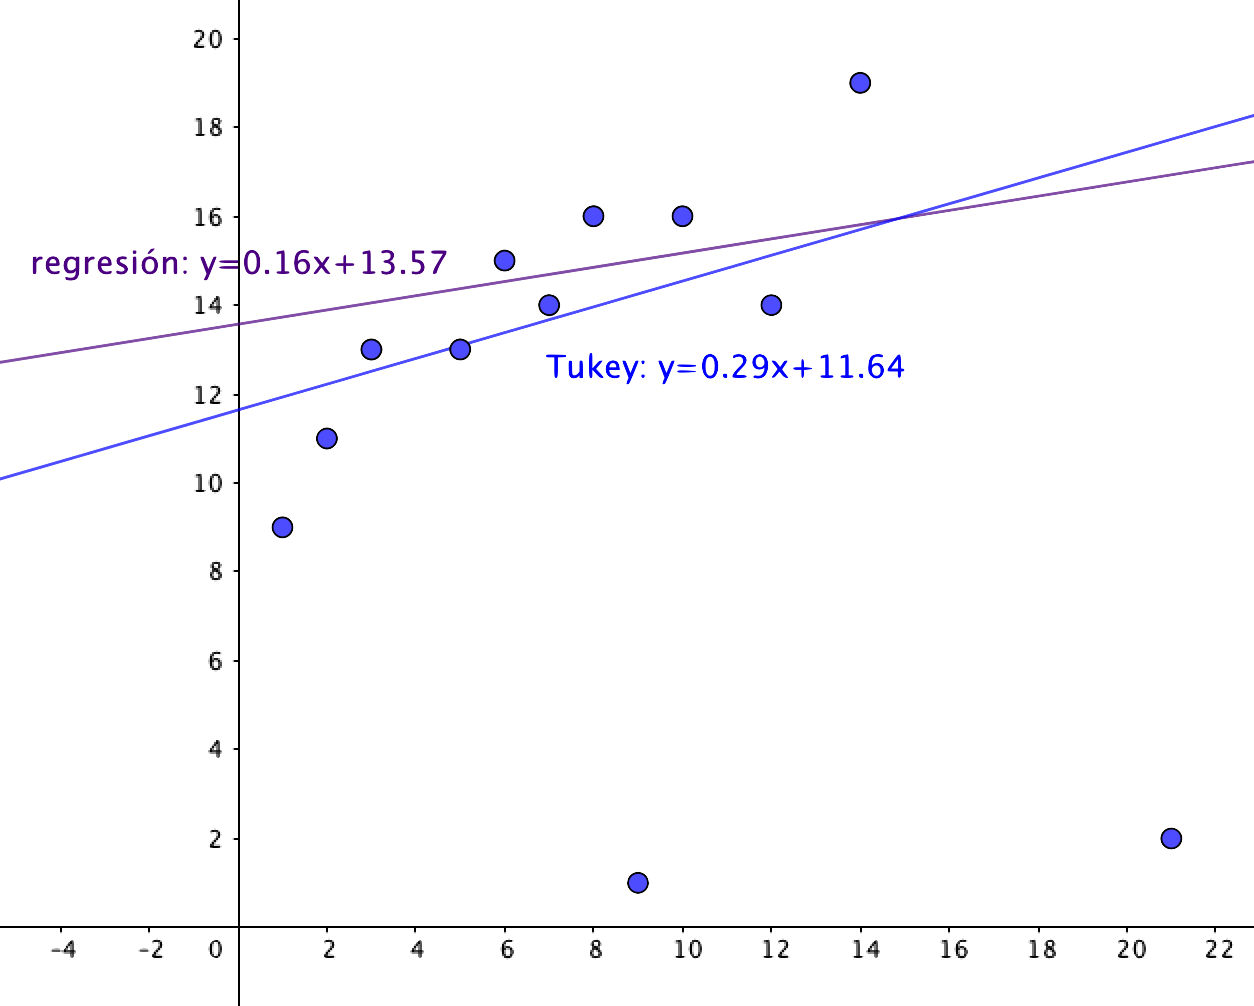
\includegraphics[width=0.75\textwidth]{imagenes/imagenes03/T03IM14.png}
	\end{figure}
Como se puede observar, la recta de regresión (morada) se ajusta muy mal al diagrama de dispersión. En cambio, la recta de Tukey se ajusta mejor, sobre todo si obviamos mentalmente los puntos que están muy aislados de la nube (los señalados en rojo en la tabla).	
	
\vspace{2mm} Se deja como ejercicio para el/la lector/a el encontrar la recta de regresión de Y sobre X: $\ y=0.16x+13.57$

\vspace{5mm} \underline{Vamos con la recta de Tukey}:

 
\begin{enumerate}
\item Se ordenan los datos en orden creciente de las abcisas (ya lo tenemos).
\item Se divide el conjunto de datos ordenados en tres grupos:

$\qquad G1=\{(1,9),\ (2,11),\ (3,13),\ (5,13) \}$

$\qquad G2=\{(6,15),\ (7,14),\ (8,16),\ (9,1) \}$

$\qquad G3=\{(10,16),\ (12,14),\ (14,19),\ (21,2) \}$



\item Para cada grupo $G_i$ se calculan las medianas de las abcisas (x) y de las ordenadas (y) del grupo, $me_{x_i}$ y $me_{y_i}$.


$G1: \ \left.
\begin{cases}
\quad \text{Abcisas   G1:} & 1,\ 2,\ 3,\ 5 \ \ \to \ m_{x_1}=2.5	 \ 
\\
\quad \text{Ordenadas G1:} & 9, 11, 13, 11 \ \to \ m_{y_1}=12	\ 
\end{cases} \ \right\}  \quad  \Rightarrow \ P1(2,5,12) $

$G2: \ \left.
\begin{cases}
\quad \text{Abcisas   G2:} & 6,\ 7,\ 8,\ 9 \ \ \to \ m_{x_2}=7.5	
\\
\quad \text{Ordenadas G2:} & 1, 14, 15, 16 \ \to \ m_{y_2}=14.5	
\end{cases} \ \right\}  \quad  \Rightarrow \ P2(7,5,14.5) $

$G2: \ \left.
\begin{cases}
\quad \text{Abcisas   G3:} & 10, 12, 14, 21 \ \ \to \ m_{x_3}=13 	
\\
\quad \text{Ordenadas G3:} & 2, 14, 16, 29 \ \ \ \to \ m_{y_3}=15	
\end{cases} \ \right\}  \quad  \Rightarrow \  P3(13,15) $

\vspace{2mm} Obsérvese que el número de datos en este caso es N = 12, múltiplo de 3, y, por tanto, cada grupo está formado por 4 datos. 

\vspace{2mm} Si el número de datos N no es múltiplo de 3, puede ocurrir que:

--- Sea múltiplo de 3 más 1; en este caso, el grupo G2 se deja con un dato más.

--- Sea múltiplo de 3 más 2; en este caso, el grupo G2 se deja con un dato menos, se añaden un dato más a los grupos G1 y G3.

\item \textbf{La recta de Tukey pasa por el baricentro del triángulo $P1P2P3$ y tiene por pendiente la de la recta que pasa por $P1$ y por $P3$}.

\vspace{2mm}  Baricentro: $B_{P1P2P3}=\dfrac{P1+P2+P3}{3}=(7.67,13.83)$

\vspace{2mm}  Pendiente: $m_{P1P3}=\dfrac{15-12}{13-2.5}=0.29$

\vspace{2mm}  Luego, la \underline{recta de Tukey} es: $\ \boldsymbol{y=0.29x+13.83}$

\end{enumerate}
\end{example}



\begin{myalertblock}{Regresiones no lineales}


El modelo de regresión lineal, estudiado para detectar dependencia lineal entre las variables, también se puede aplicar para detectar otros tipos de dependencia no lineales, como la exponencial o la potencial.

\begin{theorem}
.	\textbf{Dependencia exponencial}

Si dos variable se sospecha que están relacionadas por un modelo exponencial: $\ y=ke^{ax}$, tomando logaritmos: $\ \ln y=ax+b$, con $\ k=e^b\ \textcolor{gris}{(b=\ln k)}$.

Para encontrar una dependencia exponencial en una serie de datos $(x_i, y_i, n_i)$, buscaremos una dependencia lineal en la serie $(x_i, \ln y_i, n_i)$. Si la dependencia lineal es $Y=aX+b$, la dependencia exponencial será $Y=Ke^{aX}$, con $K=e^b$
\end{theorem}

\begin{example}
. Encontar la dependencia exponencial para los siguientes datos (X habitantes del mundo, en millones; Y año):

\begin{table}[H]
\centering
\begin{tabular}{l|rrrrrr}
X & 1750 & 1800 & 1850 & 1900 & 1950 & 2000 \\ \hline
Y & 728 & 949 & 1171 & 1608 & 2516 & 5923
\end{tabular}
\end{table}

Cálculos: 

$\ \Sigma x=11250;\ \Sigma y=12895;\ \sigma x^2=21137500;\ \Sigma y^2=46799675;\ \Sigma x\cdot y=24955950$

$\bar x=1875;\ s_x=85.39;\quad \bar y=2149.17;\ s_y=1783.54; \qquad s_{xy}=129631.25$

$r=0.85;\qquad $ Recta de regresión de Y sobre X: $\ y=17.78x-31183.33$

\vspace{4mm} Tomando logaritmos en la población (Y):

Ahora, $\ \Sigma y=43,33;\ \Sigma y^2= 314.01;\ \Sigma x\cdot y=81450.40$

Luego $\bar y=7.22;\ s_y=0.45; \ s_{xy}=37.58$

$r=0.98$. Recta de regresión de ln Y sobre X: $\ \ln y=0.0052x-7.69$

\vspace{4mm} Por último, la dependencia exponencial será: 

$y=e^{0.0052x-7.69}=e^{0.0052x}\cdot e^{-7.69}=0.00046 e^{0.0052 x}$


	\begin{figure}[H]
			\centering
			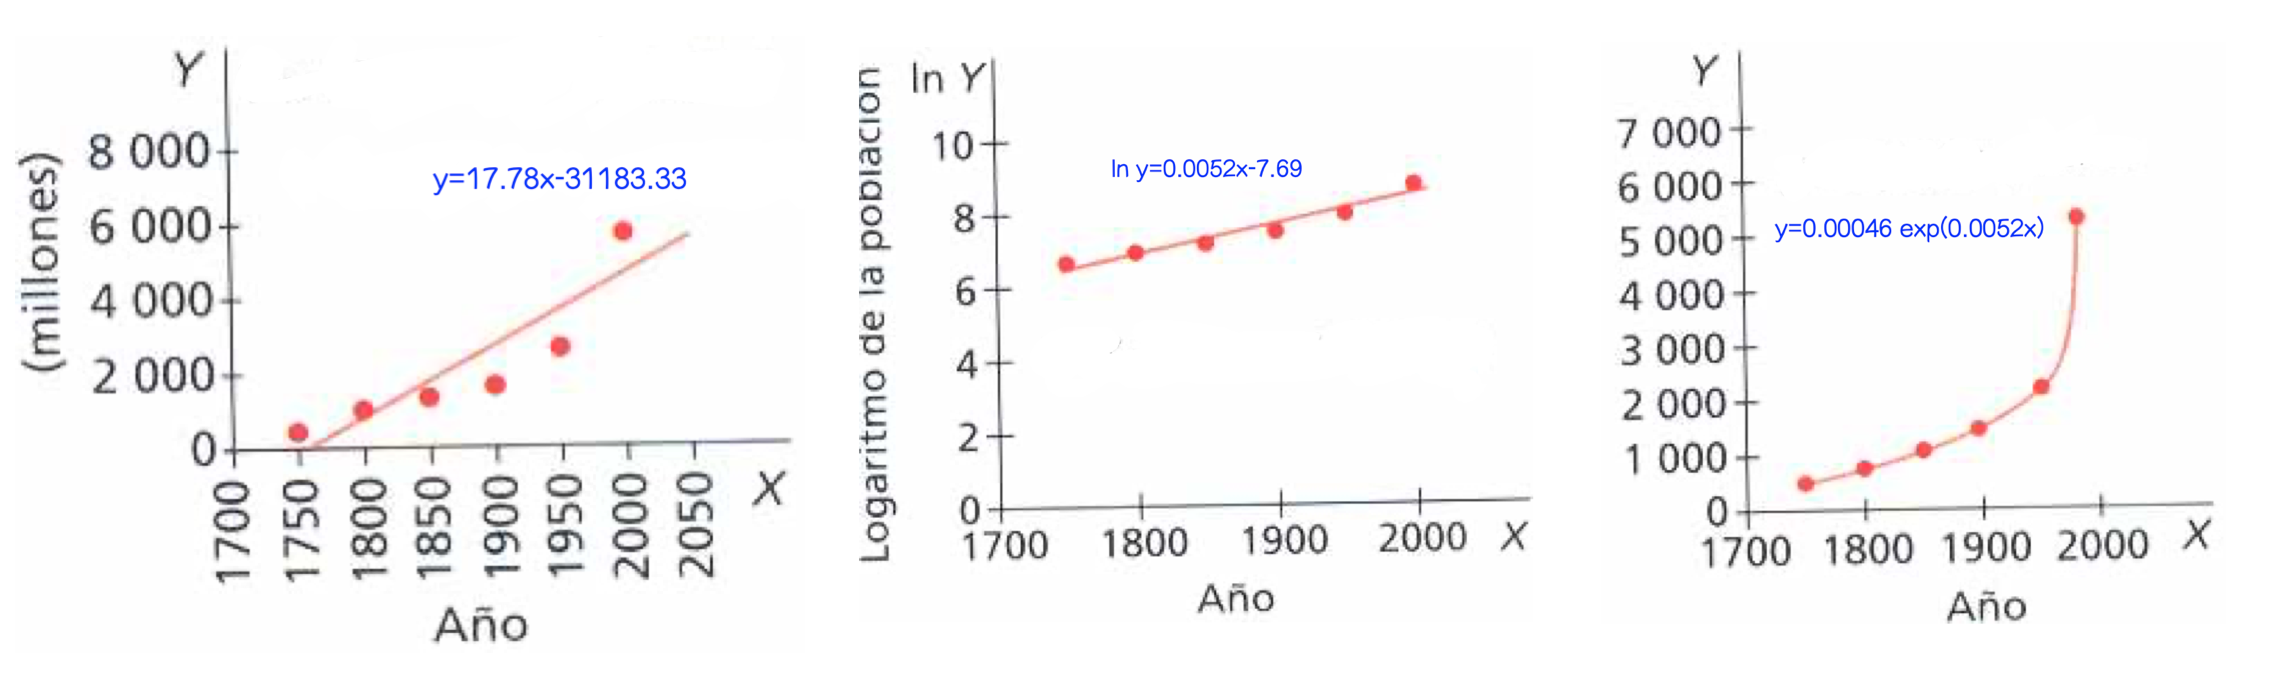
\includegraphics[width=0.95\textwidth]{imagenes/imagenes03/T03IM15.png}
			\caption*{\textcolor{gris}{\footnotesize{Ejemplo tomado de ``https://yoquieroaprobar.es/\_pdf/04140.pdf''}}}
	\end{figure}
\end{example}

\begin{theorem}
.	\textbf{Dependencia potencial}

\vspace{2mm} Si dos variables estadísticas X e Y están relacionadas por un modelo potencial: $\ y=k\ a^x$, con $k > 0$, al tomar logaritmos, se obtiene:
$\ \ln y = \ln k + a ln x$ de donde se deduce que las variables ($\ln X, \ \ln Y)$ están relacionadas por un modelo lineal.

\vspace{2mm} Para encontrar dependencia potencial en una lista de datos $(x_i, y_i, n_i)$, se aplica una regresión lineal a los datos: $(\ln x_i,\ \ln yÑi,\ n_i)$.

\vspace{2mm} Si la recta de regresión es $ln Y = a \ln X + b$, entonces la dependencia potencial en los datos originales es: $y=k\ a^x$, con $k=e^b$ .	

\vspace{2mm} Veremos un \textbf{ejemplo} que aclare todo esto.
\end{theorem}

\begin{example}
.	El científico inglés Fry Richardson midió la costa oeste de Gran Bretaña con ``reglas'' de distintos tamaños, y obtuvo los siguientes datos aproximados \textcolor{gris}{(principio de los fractales)}:	

\vspace{2mm} Calcula el coeficiente de correlación para estos datos y también para los datos $(\ln X, \ln Y)$. Compara los resultados. ?Cuál es la ley que mejor describe la dependencia entre las variables X e Y?

\begin{table}[H]
\centering
\begin{tabular}{l|lcccccc}
\textbf{Tamaño de la regla (cm)} &  & 1000 & 500 & 200 & 100 & 30 & 10 \\ \hline
\textbf{Longitud de la costa (Km)} &  & 1000 & 1000 & 1200 & 1500 & 2100 & 2800
\end{tabular}
\end{table}

Para los datos $(X, Y)$, se encuentra (hágase) que $r = –0,698$. En cambio, para los datos $(\ln x, \ln y)$ tenemos que $r = 0,985$, mucho más elevado que el anterior, y la recta de regresión es: $\ln y = –0,24 \ln x + 8,446 \ \to \ $$y=e^{-0.24 \ln x +8.46}= e^{8.46}\ x^{-0.24}= 4656.4 \ x^{-0.24}$

	\begin{figure}[H]
			\centering
			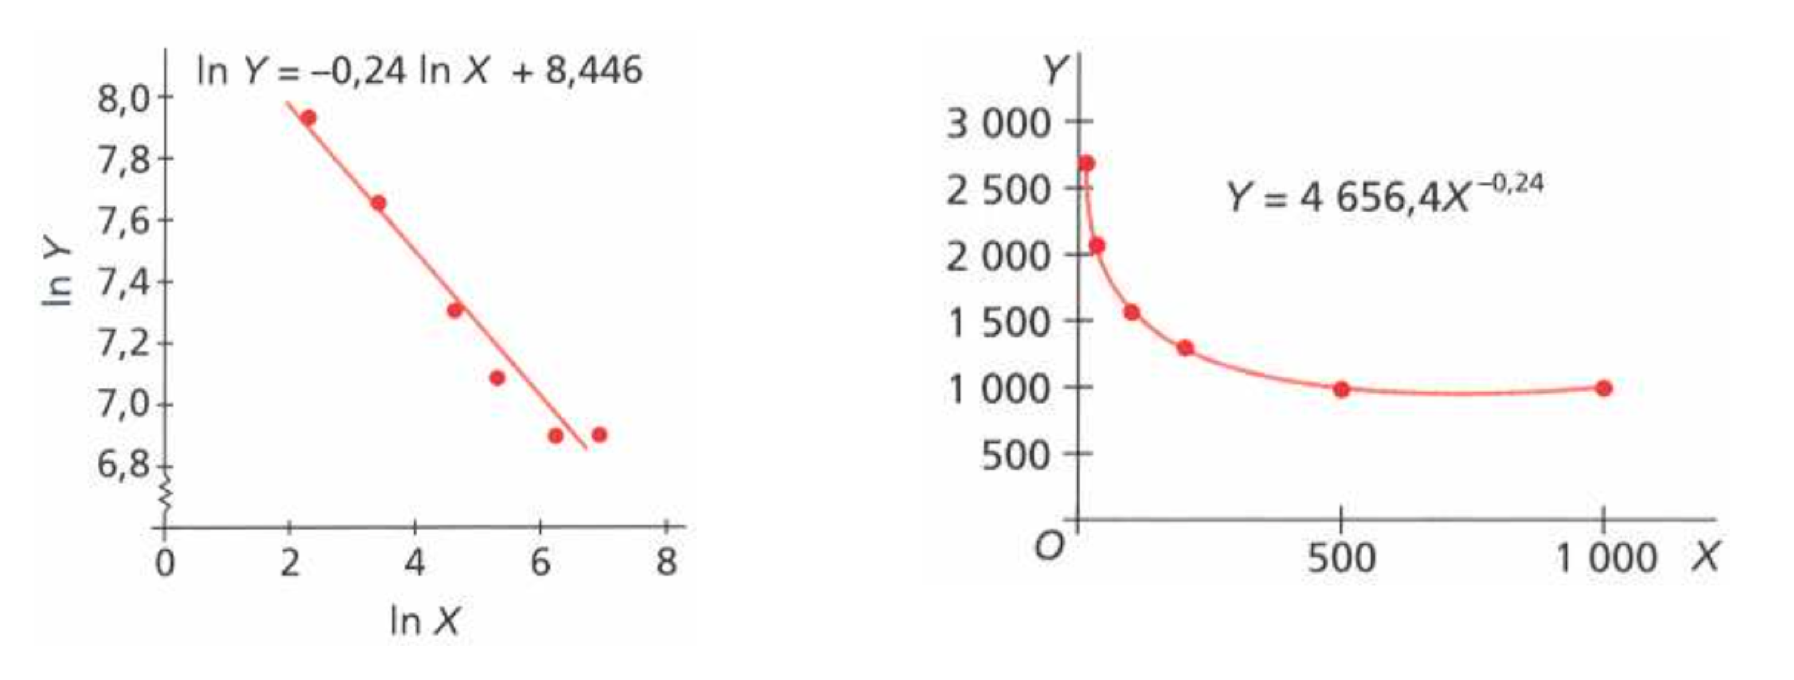
\includegraphics[width=0.75\textwidth]{imagenes/imagenes03/T03IM16.png}
			\caption*{\textcolor{gris}{\footnotesize{Ejemplo tomado de ``https://yoquieroaprobar.es/\_pdf/04140.pdf''}}}
	\end{figure}

\end{example}
\end{myalertblock}


\section{Ejercicios}

$$\subrayado{\  \boxed{ \textbf{Se deberían intentar resolver los ejercicios antes de ver su resolución.} \ } \ }$$

\vspace{1cm} %******************************************

\begin{ejemplo}
\begin{ejer}\textcolor{white}{.}

Se ha hecho una encuesta a 12 personas que han tenido un accidente de tráfico, preguntando por el número de meses transcurridos e incluyendo el grupo de edad. 

Las respuestas han sido: 

Carmen, 35: [60, 70);  Teresa, 15: [50, 60);  Pilar, 12: [50, 60);  Esther, 6: [20, 30); Juan, 8: [40, 50); Jacinto, 15: [30, 40); Jesús, 24: [50, 60); Marta, 12: [30, 40); José, 28: [40, 50); Andrés, 3: [20, 30); María Jesús, 20: [40, 50); Beatriz, 16: [30, 40) 

\begin{adjustwidth}{20pt}{10pt}
\begin{enumerate}[a) ]
\item Construye la tabla correspondiente a la variable bidimensional.
\item  Representa el diagrama de dispersión. 
\item Estudia si hay correlación entre ambas variables, y determina su coeficiente de correlación lineal.	
\item Si la persona entrevistada tuviese 87 años, ?`cuántos meses es de esperar que hayan transcurrido desde su último accidente?
\item Si a un encuestado le han transcurrido 18 meses desde su último accidente, ?`qué edad es de esperar que tenga?
\item Como de fiables son tus predicciones.
\end{enumerate}
\end{adjustwidth}
\end{ejer}
\end{ejemplo}

--- a) Representamos los datos en una tabla de doble entrada:

\begin{table}[H]
\centering
\begin{tabular}{|c|c|c|c|c|c|c|c|c|c|c|c|}
\hline
\textbf{Y   \textbackslash   X} & \textbf{3} & \textbf{6} & \textbf{8} & \textbf{12} & \textbf{15} & \textbf{16} & \textbf{20} & \textbf{24} & \textbf{28} & \textbf{35} & \textbf{total} \\ \hline
\textbf{$\boldsymbol{[20,30[\to 25}$} & 1 & 1 &  &  &  &  &  &  &  &  & \textit{2} \\ \hline
\textbf{$\boldsymbol{[30,40[\to 35}$} &  &  &  & 1 & 1 & 1 &  &  &  &  & \textit{3} \\ \hline
\textbf{$\boldsymbol{[40,50[\to 45}$} &  &  & 1 &  &  &  & 1 &  & 1 &  & \textit{3} \\ \hline
\textbf{$\boldsymbol{[50,60[\to 55}$} &  &  &  & 1 & 1 &  &  & 1 &  &  & \textit{3} \\ \hline
\textbf{$\boldsymbol{[60,70[\to 65}$} &  &  &  &  &  &  &  &  &  & 1 & \textit{1} \\ \hline
\textbf{totales} & \textit{1} & \textit{1} & \textit{1} & \textit{2} & \textit{2} & \textit{1} & \textit{1} & \textit{1} & \textit{1} & \textit{1} & \textbf{12} \\ \hline
\end{tabular}
\end{table}

--- b) Diagrama de dispersión:

	\begin{figure}[H]
			\centering
			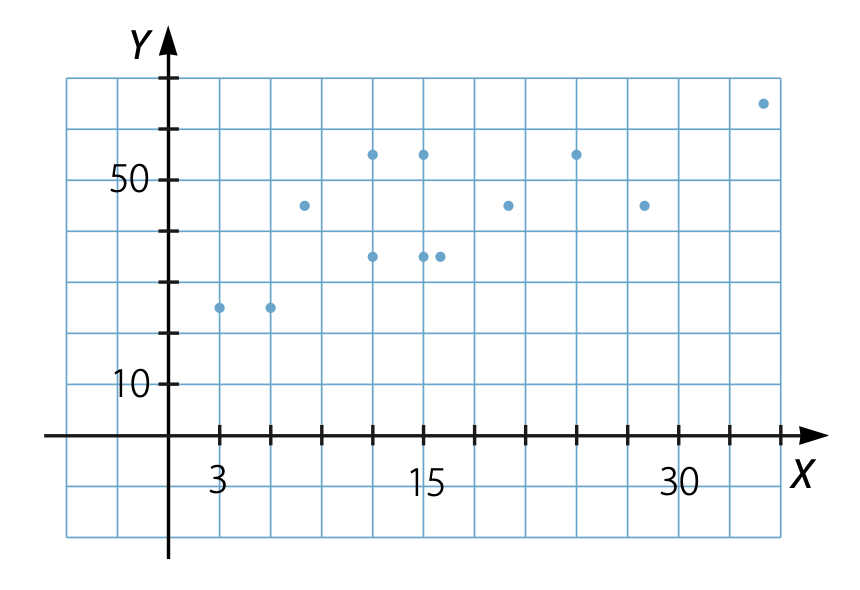
\includegraphics[width=0.75\textwidth]{imagenes/imagenes03/T03IM17.png}
	\end{figure}

Se observa cierta correlación lineal positiva y no muy fuerte.

--- c) Cálculos:

	\begin{figure}[H]
			\centering
			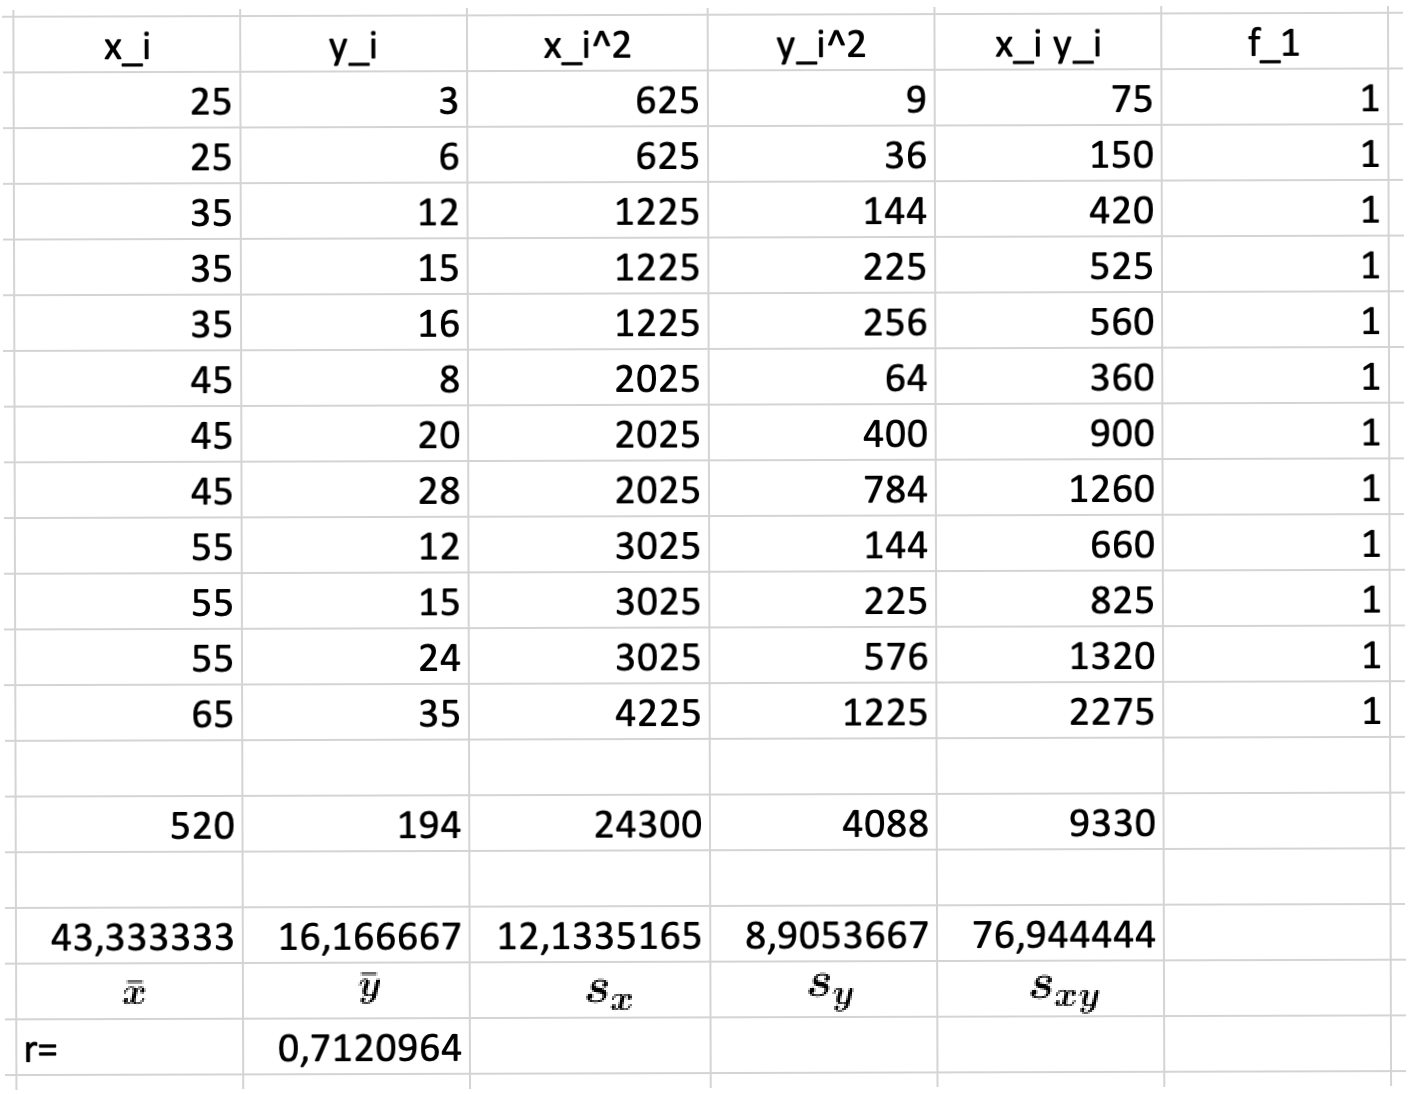
\includegraphics[width=0.8\textwidth]{imagenes/imagenes03/T03IM18.png}
	\end{figure}
	
$\bar x=43,3$ años; $\ \ \bar y=16.2$ meses; $\ \ s_x=12.1$; $\ \ s_y=8.9$; $\ \ s_{xy}=76.9 \ \to \ r=0.71$. Hay una correlación positiva y no muy fuerte.

--- e) Para $x=87$ años $\ \to \ $ 

Necesitamos la recta de regresión de Y sobre X: 

$y-16.17=\dfrac{76.94}{12.13^3}\ (x-43.3) \ \to \ y= 0.52x-6.48$

$x=87$ años $\ to \ y=38.76$, casi 39 meses.

--- f) Para $y=18$ meses $\ \to \ $


Necesitamos la recta de regresión de X sobre Y:

$x-43.33=\dfrac{76.94}{8.91^2}\ (y-16.17) \ \to \ x=0.97y+27.66$

$y=18$ meses $\ \to \ x=45.12$, 45 años aproximadamente.

--- g) Al no ser muy fuerte la correlación ($r=0.71$), las estimaciones que hemos hecho no son  muy fiables, siendo la primera (87 años $\to$ 39 meses) mucho menos fiable a tratarse de una extrapolación (nuestros datos abarcan edades desde 20 hasta 70 años).




\vspace{5mm} %***************************************
\begin{ejemplo}
\begin{ejer}\textcolor{white}{.}
	La recta de regresión de una variable Y respecto de la variable X es $y = 0,3x + 1$. Los valores que ha tomado la variable $x$ han sido $\{3, 4, 5, 6, 7\}$.
	
\begin{adjustwidth}{20pt}{10pt}
 \begin{enumerate}[a) ]
 	\item Determina el valor esperado de $y$ para el valor particular de $x = 3.5$.
 	\item Si los valores de la variable Y utilizados para la regresión se multiplican por 10 y se dejan los mismos valores para la variable X, determina razonadamente la nueva recta de regresión.
 \end{enumerate}
 \end{adjustwidth}
	
\end{ejer}
\end{ejemplo}

--- a) $x=3.5 \ \to \ y=0.3\cdot 3.5+1=2.05$

--- b) $Y':\ 10\cdot y_i \to \bar y'=10 \bar y$
$;\quad$
$S'_{XY}=	\dfrac {\displaystyle \sum_{i=1}^N x_i \ 10 y_i \ n_i}{N}-\bar x \cdot 10 \bar y = 10 s_{xy}$

$ y - 10 \bar y= \dfrac {10 s_{xy}}{s_x^2}\ (x-\bar x) \ \to \ 
y=10\ \dfrac{s_{xy}}{s_x^2} \ x+ 10 \left(\bar y - \dfrac {s_{xy}}{s_x^2} \right) =3x+10$


\vspace{5mm} %***************************************
\begin{ejemplo}
\begin{ejer}\textcolor{white}{.}
	Cien alumnos prepararon un examen de Matemáticas. Se representa por X el número de problemas hechos por cada alumno en la preparación, y por Y, la calificación obtenida. Sabiendo que las medias aritméticas de esas variables fueron $\bar x= 9.2$ e $\bar y= 9.5$, que el coeficiente de correlación entre esas variables fue $0.7$ y que la desviación típica de la variable Y fue el doble que la de la variable X, calcula las ecuaciones de las rectas de regresión.
\end{ejer}
\end{ejemplo}

$s_y=2s_x \ \to \ r=\dfrac{s_{xy}}{s_x\ s_y}= \dfrac{s_{xy}}{2 s_x^2}=0.7 \ \Rightarrow \ \dfrac{s_{xy}}{s_x^2}=1.4$

$y-\bar y=\dfrac{s_{xy}}{s_x^2}\ (x-\bar x) \ \ \Rightarrow \ \ y-9.5=1.4\ (x-9.2)$

$\dfrac{s_xy}{s_y^2}=\dfrac{s_{xy}}{(2s_x)^2}=\dfrac 1 4 \ \dfrac{s_{xy}}{s_x^2}=\dfrac 1 4 \ \dfrac 1.4 =0.35$

$x-\bar x=\dfrac{s_{xy}}{s_y^2}\ (y-\bar y) \ \ \Rightarrow \ \ x-9.2=0.35\ (y-9.5)$





 
\subsection{Problemas propuestos (con solución)}



\begin{adjustwidth}{20pt}{10pt}
\begin{enumerate}[PB. 1. ]

\item En cada uno de estos casos debes decir si, entre las dos variables que se citan, hay relación funcional o estadística (correlación) y, en este último caso, indicar si es positiva o negativa:

	\begin{enumerate}[a) ]
	\item En un conjunto de familias: estatura media de los padres -- estatura media de los hijos.
	\item Entre los países del mundo respecto a España: volumen de exportación -- volumen de importación.
	\item En los países del mundo: tasa de mortalidad infantil -- médicos por cada 1 000 habitantes.
	\item En las viviendas de una ciudad: kw consumidos en un mes -- coste del recibo de la luz.
	\item En los equipos de fútbol: posición al finalizar la liga -- número de partidos perdidos.
	\end{enumerate}

\hspace{-1cm}\rotatebox{180}{\leftline{\textcolor{gris}{E+, E-, E-, F+, E+}}}\vspace{1cm}



\item Dados los coeficientes de correlación: $\ r_1=0.64; \ r_2=0.95;\ r_3=-1; \ r_4=-0.76$; asocia cada uno de ellos a las siguientes nubes de puntos.

	\begin{figure}[H]
			\centering
			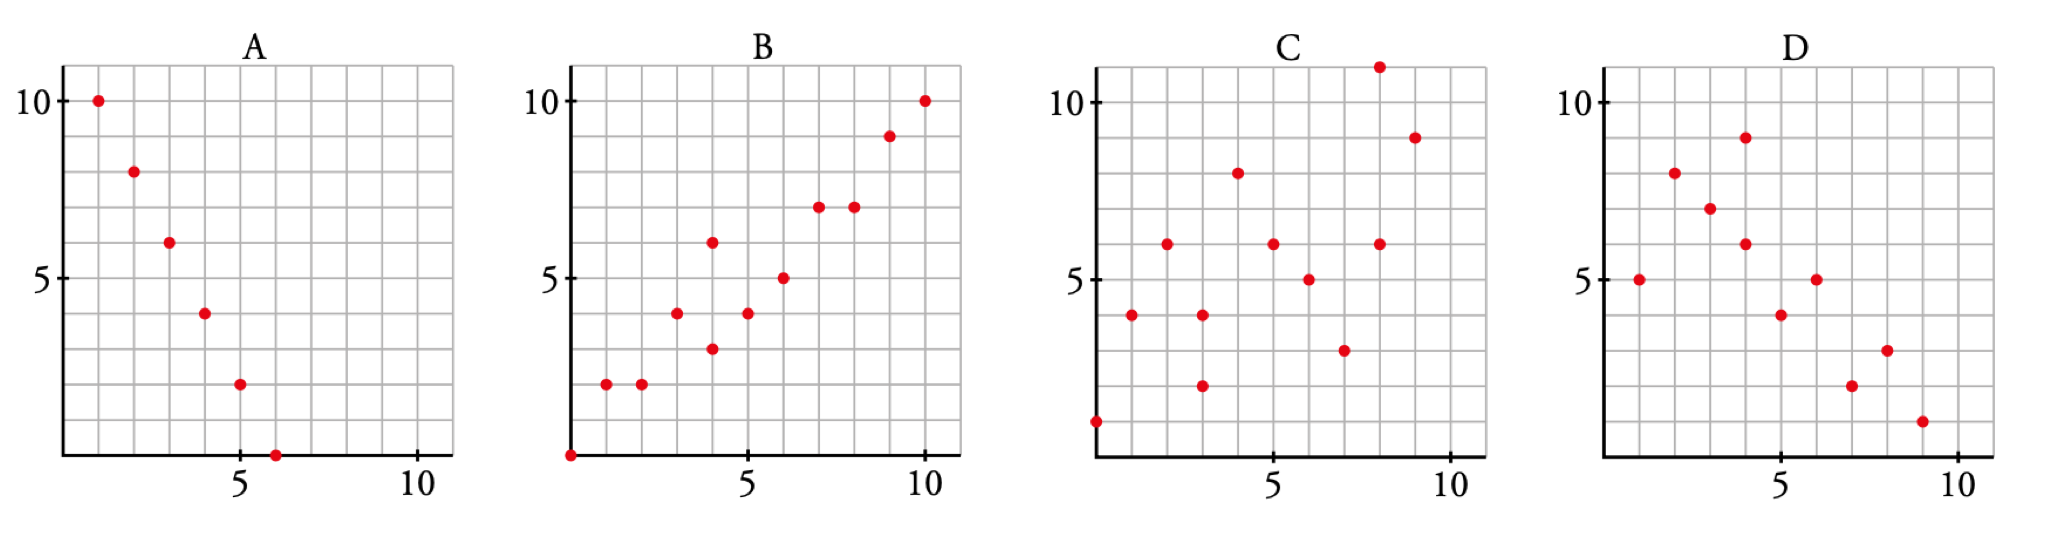
\includegraphics[width=0.95\textwidth]{imagenes/imagenes03/T03IM19.png}
	\end{figure}
 
\hspace{-1cm}\rotatebox{180}{\leftline{\textcolor{gris}{$r_1\to C;\ r_2\to B;\ r_3\to A;\ r_4\to D$}}}\vspace{1cm}





\item Dados los coeficientes de regresión $\ r_1=-0.9;\ r_2=0.99;\ r_3=0.6;\ r_4=-0.2;\ r_5=-0.5; \ r_6=0.1$ y las rectas de regresión de la siguiente figura, asocia por parejas.

\begin{figure}[H]
			\centering
			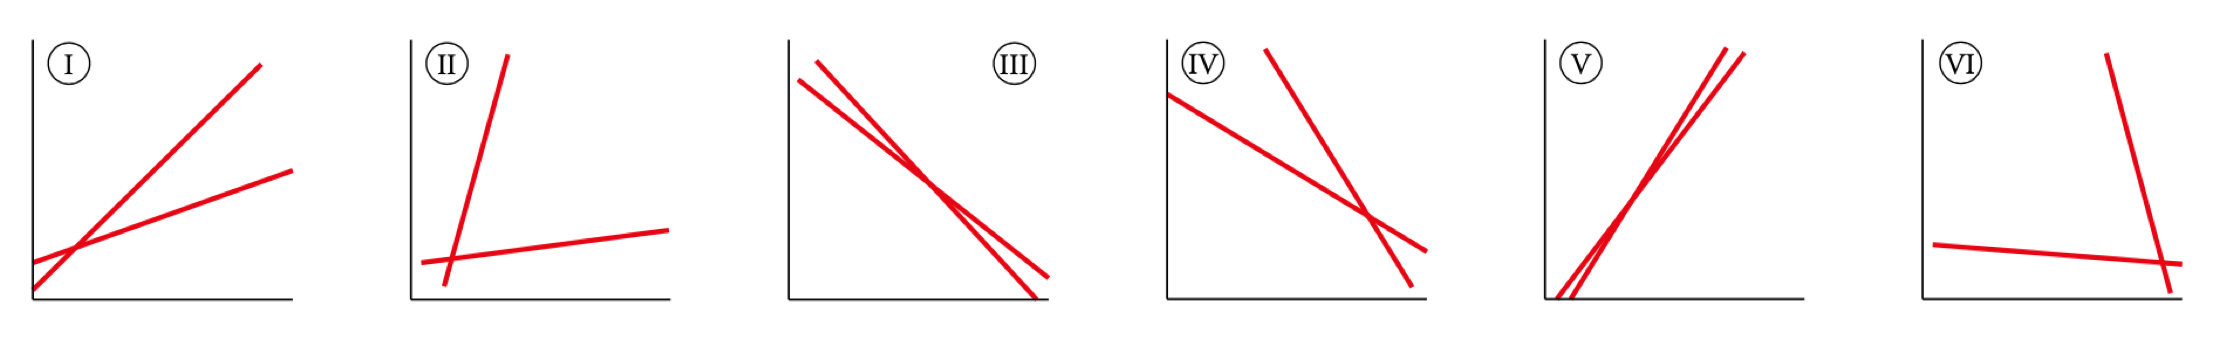
\includegraphics[width=0.95\textwidth]{imagenes/imagenes03/T03IM20.png}
	\end{figure}

 
\hspace{-1cm}\rotatebox{180}{\leftline{\textcolor{gris}{$I\to r_3;\ II\to r_6;\ III\to r_1;\ IV\to r_5;\ V\to r_2;\ VI\to r_4$}}}\vspace{1cm}





\item Un excursionista, en diez marchas distintas, toma las siguientes medidas: x -- altura de lugar (en m); y -- presión atmosférica (en mm Hg); z -- número de pulsaciones en reposo.

\begin{table}[H]
\centering
\begin{tabular}{|c|r|r|r|r|r|r|r|r|r|r|}
\hline
\textbf{x} & 0 & 184 & 231 & 481 & 730 & 911 & 1343 & 1550 & 1820 & 2184 \\ \hline
\textbf{y} & 760 & 745 & 740 & 720 & 700 & 685 & 650 & 630 & 610 & 580 \\ \hline
\textbf{z} & 73 & 78 & 75 & 78 & 83 & 80 & 89 & 80 & 85 & 92 \\ \hline
\end{tabular}
\end{table}

Halla el coeficiente de correlación y la recta de regresión para la distribución x-y y para x-z y analiza los resultados.
 
\hspace{-1cm}\rotatebox{180}{\leftline{\textcolor{gris}{$r_{xy}=-0.99;\ y=-0.08x+759;\quad r_{xz}=0.85;\ z=6.87x+74.8$}}}\vspace{1cm}




\item La recta de regresión de Y sobre X de una distribución bidimensional es $y = 1.6 x - 3$. Sabemos que $\bar x = 10$ y $r = 0.8$.

Calcula $\bar y$ y estima el valor de $y$ para $x = 12$ y para $x = 50$. 

?`Qué estimación te parece más fiable?
 
\hspace{-1cm}\rotatebox{180}{\leftline{\textcolor{gris}{$(\bar x,\bar y)\in r: \to \bar y=13;\quad y(12)=16.2;\ y(50)=77; \quad $ }}}

\hspace{-1cm}\rotatebox{180}{\leftline{\textcolor{gris}{Primera estimación más fiable; 12 más próximo a $\bar x$ que 50.}}}\vspace{1cm}




\item Considera la siguiente variable bidimensional:

\begin{table}[H]
\centering
\begin{tabular}{|c|r|r|r|r|r|r|r|r|r|}
\hline
\textbf{x} & 1 & 2 & 3 & 4 & 5 & 6 & 7 & 8 & 9 \\ \hline
\textbf{y} & 5 & 6 & 8 & 11 & 1 & 13 & 14 & 14 & 17 \\ \hline
\end{tabular}
\end{table}

Encuentra la recta de regresión de Y sobre X y la recta de Tukey.
 
\hspace{-1cm}\rotatebox{180}{\leftline{\textcolor{gris}{Regresión:$y=1.43x+2.74;\qquad $ Tukey: $y=1.33x+3.67$}}}\vspace{1cm}




\item Dada la siguiente variable bidimensional, encuentra la recta de regresión de Y sobre X y la recta de Tukey.

\begin{table}[H]
\centering
\begin{tabular}{|c|r|r|r|r|r|r|r|r|r|r|}
\hline
\textbf{x} & 1 & 2 & 3 & 4 & 5 & 6 & 7 & 8 & 9 & 10 \\ \hline
\textbf{y} & 7 & 8 & 6 & 8 & 1 & 10 & 9 & 7 & 8 & 11 \\ \hline
\end{tabular}
\end{table}
 
\hspace{-1cm}\rotatebox{180}{\leftline{\textcolor{gris}{Regresión:$y=0.32x+5.33;\qquad $ Tukey: $y=0.14x+6.23$}}}\vspace{1cm}



\item Para una variable bidimensional se conoce $r = -0.5,\;  s_x = 2; \text{ y } s_y = 3$. Razona si alguna de las siguientes rectas de regresión de Y sobre X corresponde a estos datos:

$a)\ y=-x +2;\quad  b)\ y=0.5x-1; \quad  c)\ 3x+4y-4=0$

 
\hspace{-1cm}\rotatebox{180}{\leftline{\textcolor{gris}{c) \textcolor{gris}{$\quad \left( s_{xy}=r\ s_x \ s_y \ \to \ m_{YX}= \dfrac{s_{xy}}{s_x^2}=-3/4 \right)$}}}}\vspace{1cm}




\item  Las rectas de regresión de Y sobre X y de X sobre Y en una distribución bidimensional, son las siguientes:
$y = 0-91x - 5.88$;  $\ x = 0.85y + 13.24$

?`Cuál es el coeficiente de correlación de Pearson de la distribución? 
 
\hspace{-1cm}\rotatebox{180}{\leftline{\textcolor{gris}{$r = 0,879\quad $ \textcolor{gris}{$(r^2=m_{YX}\cdot m_{XY})$}}}}\vspace{1cm}



\end{enumerate}
\end{adjustwidth}



\section{Curiosidades}

\begin{myexampleblock}{Cuarteto de Anscombe}

La correlación y la regresión están relacionadas entre sí. Ahora bien, puede ocurrir que dos variables estén correlacionadas entre sí pero, en cambio, la relación entre ellas puede ser de tipo muy diferente en uno u otro caso. El estadístico inglés Frank Anscombe, ideó un conjunto de ejemplos de datos (conocido como el cuarteto de Anscombe)\footnote{\scriptsize{http://e-ducativa.catedu.es/44700165/aula/archivos/repositorio/2000/2007/html/31\_rectas\_de\_regresin\_i.html}} de tal manera que todos ellos tienen los mismos parámetros estadísticos (medias, desviaciones típicas, correlación y recta de regresión) pero, en cambio, la relación entre las variables es muy diferente entre sí: el primero sería una distribución normal (lo que cabría esperar de los parámetros), la segunda es una función no lineal, y las otras dos son lineales pero afectadas cada una por un dato que se escapa de la relación de los demás. Los diagramas de dispersión y la recta de regresión correspondiente son:

	
	
	\begin{figure}[H]
			\centering
			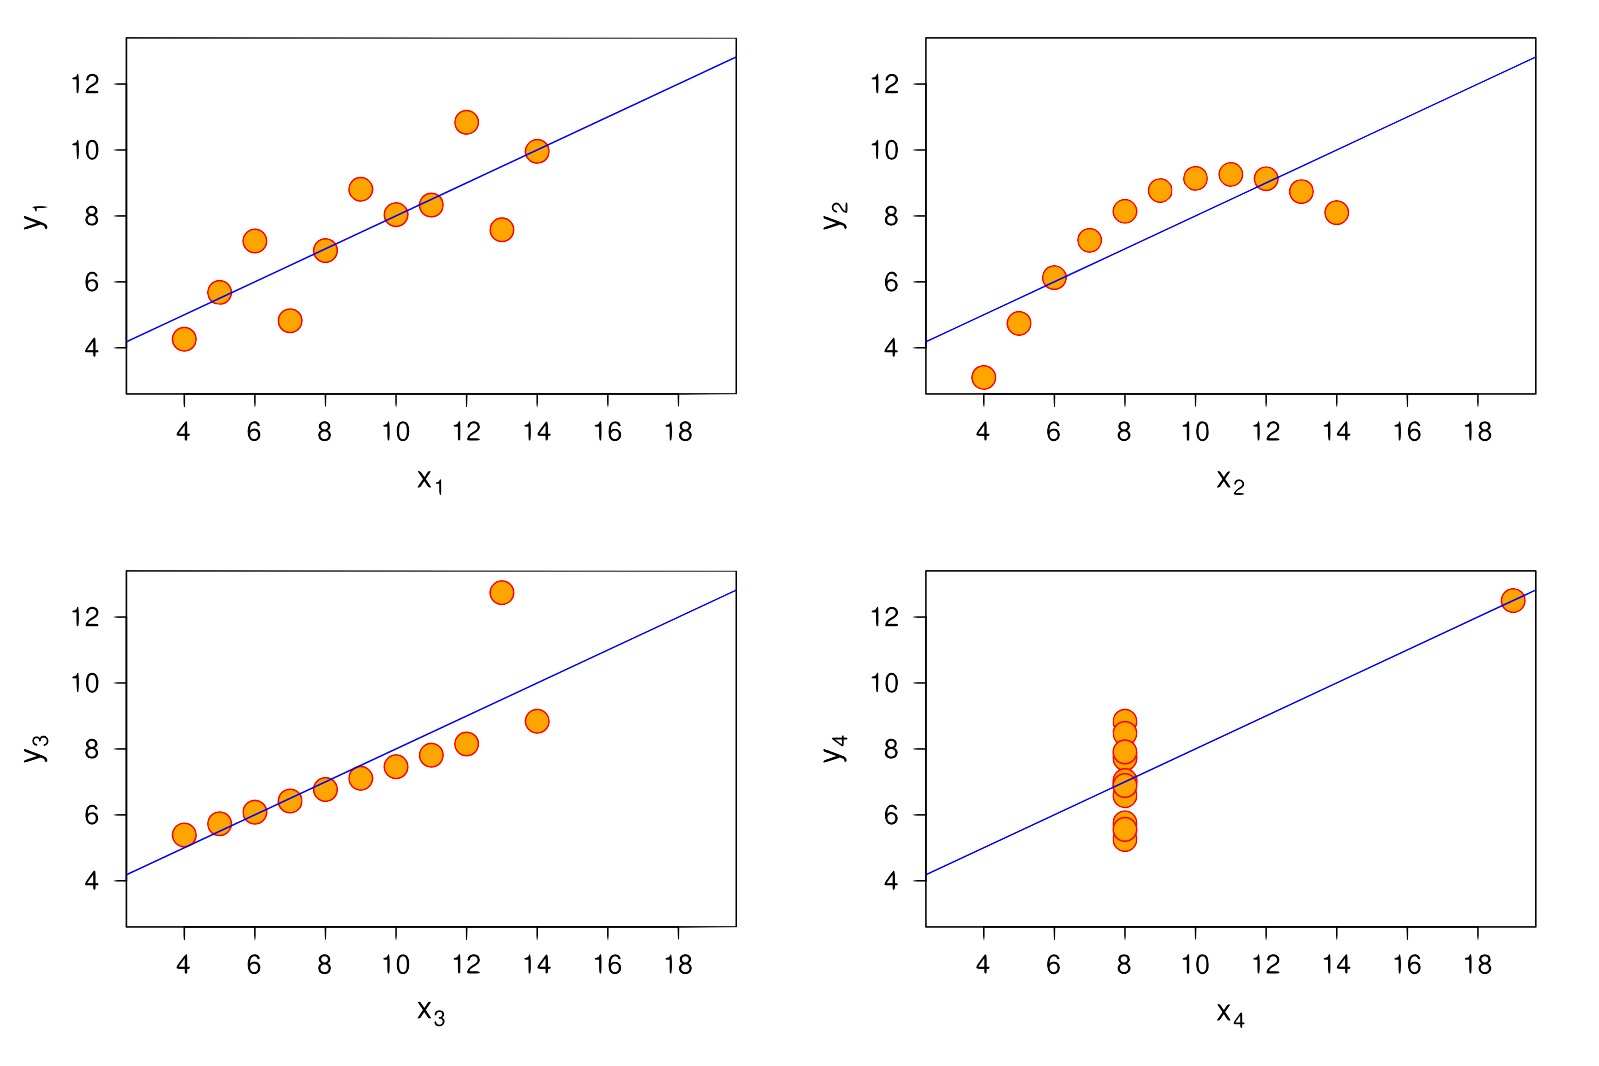
\includegraphics[width=0.95\textwidth]{imagenes/imagenes03/T03IM22.png}
	\end{figure}
	
	\vspace{-5mm}%*********************
	En este conjunto se puede apreciar claramente que es muy importante no fiarse sólo de la correlación y regresión que haya entre dos variables (aunque sea fuerte, los cuatro ejemplos tienen una correlación de 0.816) para pensar que hay una relación lineal entre las mismas. Así, en primer lugar, debemos considerar el diagrama de dispersión para, luego, estudiar los valores de la correlación y de la regresión. Los dos últimos ejemplos también nos muestran la influencia que tienen en la recta de regresión los datos aislados que se encuentran lejos del resto.

\rule{65mm}{0.1mm}
	
\begin{scriptsize}\textsf{
 Se pueden consultar las 4 distribuciones y sus parámetros coincidentes en :}
 
\vspace{-4mm}\begin{flushright}
	\textsf{``https://upload.wikimedia.org/wikipedia/commons/b/b6/Anscombe.svg'}\end{flushright}
 \end{scriptsize}

\end{myexampleblock}



\vspace{5mm} %************************************
\begin{myexampleblock}{Correlación no implica causalidad}

\begin{small}
El ejemplo más clásico de que \textbf{``Correlación ni implica causalidad’’}\footnote{Artículo de Daniel Manzano, obtuvo el primer premio del concurso DIPC de divulgación del evento Ciencia Jot Down 2016} es el de los piratas y el calentamiento global. Este se basa en un estudio desarrollado nada menos que por \textbf{Bobby Henderson}, el creador de la \emph{``Iglesia pastafari''}. Su intención era combatir los argumentos de los creacionistas, un grupo muy dado a encontrar correlaciones donde no las hay y a concluir que hay una causa detrás. 




\vspace{2mm} Casualmente la causa que siempre encuentran es la misma, `Dios causa que ...', de nuevo casualmente, coincide con lo que estaban intentando demostrar a priori. Para ilustrar el hecho de que el que dos fenómenos se den al mismo tiempo no implica que uno cause el otro. Henderson representó la temperatura global de la Tierra en función del número de piratas en el mundo.

	\begin{figure}[H]
			\centering
			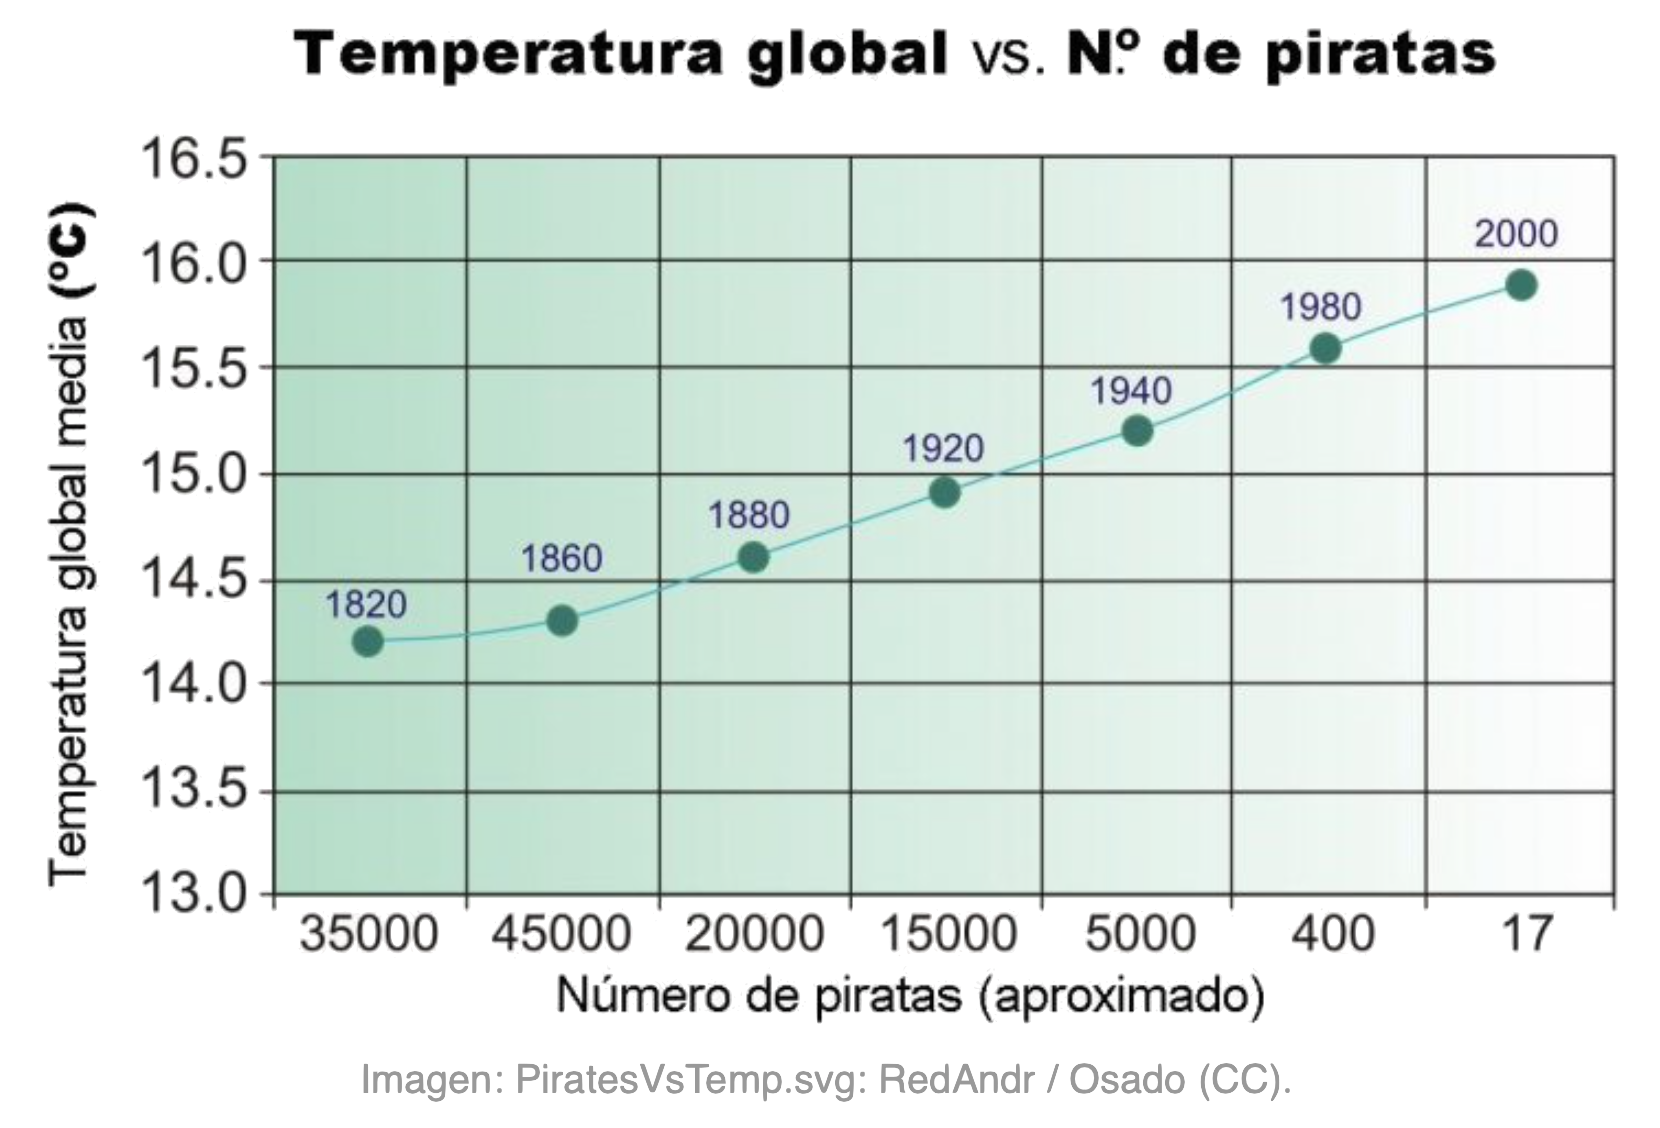
\includegraphics[width=0.6\textwidth]{imagenes/imagenes03/T03IM23.png}
	\end{figure}

Claramente se aprecia que, a medida que el número de piratas se ha reducido, la temperatura de la atmósfera ha aumentado. Según los argumentos de los creacionistas, y otros grupos favorables a encontrar causas donde no las hay, esto significaría que la escasez de piratas es la verdadera causa del calentamiento global. No hay otra explicación. Por este motivo los seguidores de la religión de Henderson se disfrazan de piratas en el momento del culto, para combatir así el cambio climático.

\vspace{2mm} Veamos otro ejemplo. La página web \textbf{``Spurious Correlations’’} (\emph{correlaciones espurias}) se dedica a buscar en distintas bases de datos correlaciones absurdas entre series de datos. Una de las más populares es la que aparece en la siguiente gráfica, que representa a través de los años tanto el número de ahogamientos en piscina producidos en los Estados Unidos como el número de películas realizadas por Nicolas Cage.

	\begin{figure}[H]
			\centering
			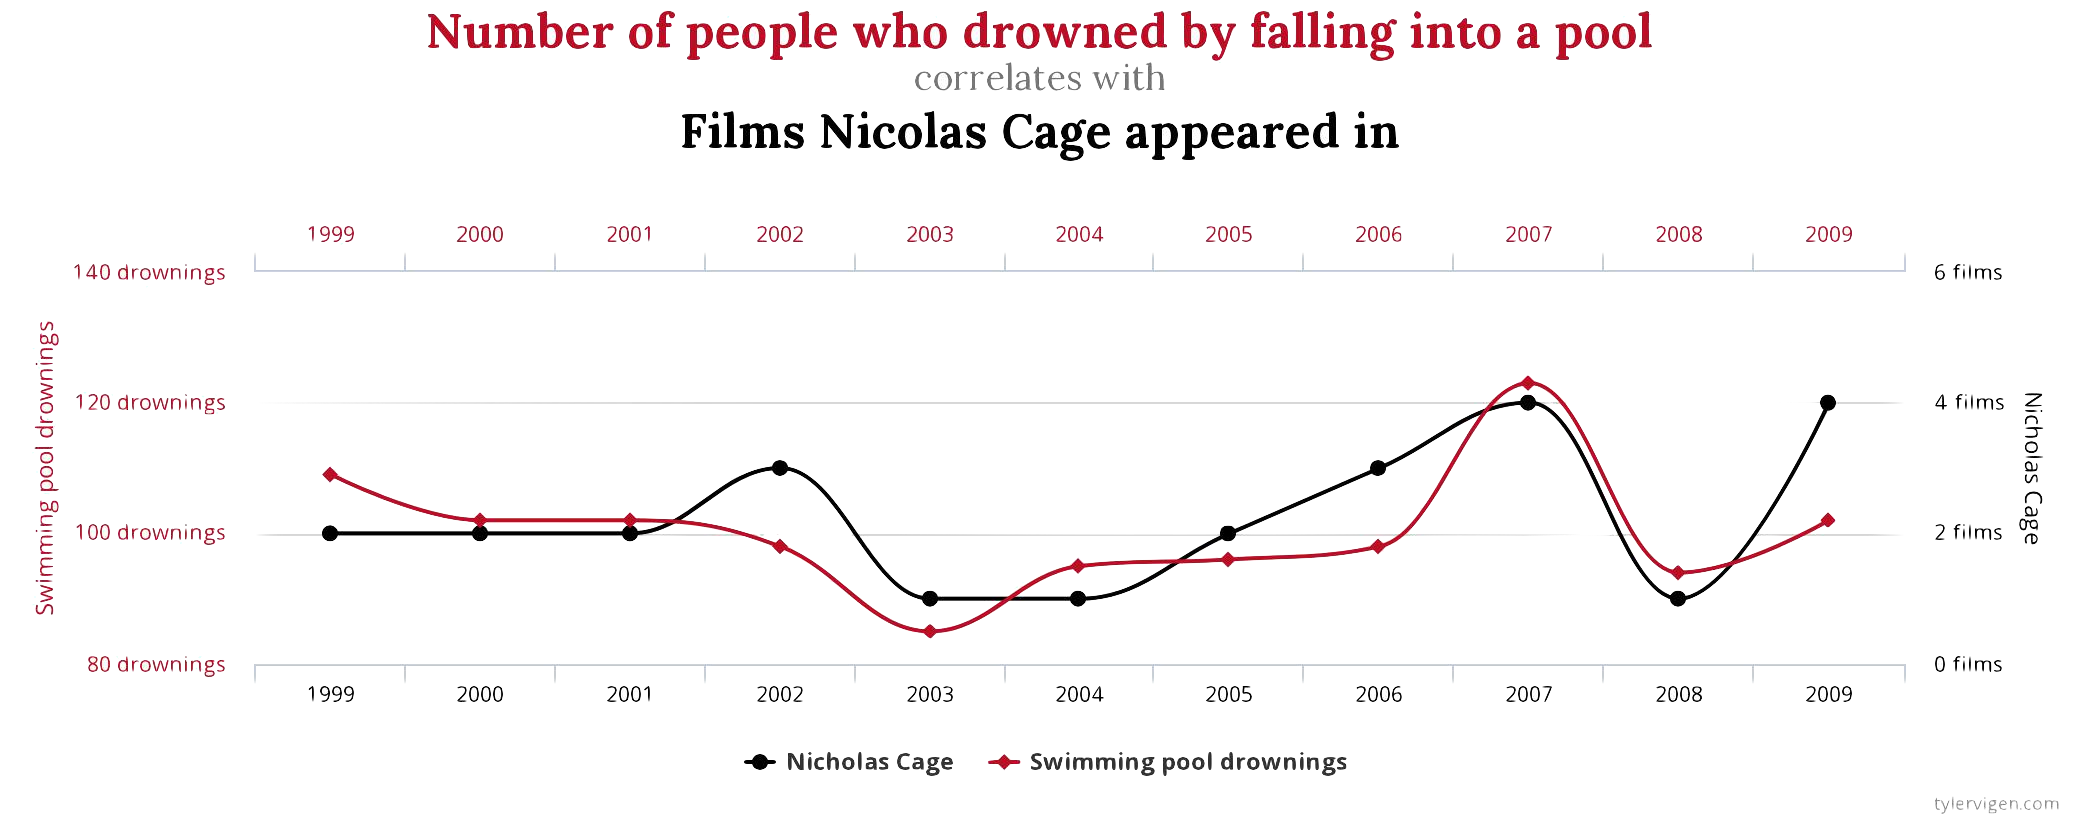
\includegraphics[width=0.95\textwidth]{imagenes/imagenes03/T03IM24.png}
	\end{figure}

La correlación es clara. Cuantas más películas hace el bueno de Nicolas más gente muere ahogada. Lo mejor será que el pobre se retire y así ahorrará sufrimiento al mundo.

\vspace{2mm} Dado que es difícil de creer que la gente se ahogue por culpa de Nicolas Cage, o que los piratas determinen la temperatura global, podemos concluir que estas correlaciones no implican que una cosa sea la causa de la otra. Veamos entonces la explicación canónica a estas gráficas. Que dos fenómenos se den a la vez, o que uno preceda al otro, no implica que uno sea la causa del otro. Aunque observamos una correlación entre A (películas de Cage) y B (ahogamientos en piscina) eso no significa que las películas de Nicolas Cage provoquen que la gente quiera morir de una manera agónica a la vez que refrescante.

\vspace{2mm} ¿`Y, si no es A la causa de B, por qué se dan los dos fenómenos a la vez de forma repetida? Bueno, en general, si hay una fuerte correlación entre los fenómenos A y B, tenemos cuatro posibilidades:

\begin{adjustwidth}{20pt}{5pt}
\textcolor{gris}{--- Que A cause B (que los ahogamientos en piscinas hagan que el bueno de Nicolas quiera hacer más cine para animar a las familias).}

\textcolor{gris}{--- Que B cause A (yo mismo estuve tentado de ahogarme después de ver La búsqueda 2).}

\textcolor{gris}{--- Que haya un tercer fenómeno, C, que provocara tanto A como B (es complicado imaginar alguno, pero a lo mejor el Orden Mundial conspira para reducir la población humana tanto mediante el ahogamiento como mediante el aburrimiento).}

\textcolor{gris}{--- Puro y duro azar. Hay muchos datos en el mundo, así que si los comparamos todos más tarde o más temprano encontraremos este tipo de correlaciones que no significan nada.}
\end{adjustwidth}

\vspace{2mm} Nadie duda de que la correlación no implica causalidad. Científicos de todos los campos dedican cantidades ingentes de tiempo a repetir experimentos para distinguir correlaciones importantes de correlaciones espurias. Incluso se ha observado que muchos experimentos científicos con grandes correlaciones tienen una probabilidad alta de ser puramente casuales. Eso ocurre porque en el mundo se realizan muchos experimentos continuamente. La probabilidad de que nunca se dé una correlación espuria es realmente baja y son precisamente las correlaciones inesperadas las que más interesan a la comunidad científica. El único remedio para evitar esto es la repetición de los experimentos. Sin embargo, todo esto no quiere decir que las correlaciones no tenga relevancia, o que no sean indicativas de causalidad. Tenemos que saber distinguir entre correlaciones más y menos probables. Tenemos que analizar cada caso cuantitativamente y averiguar cuál es la probabilidad de que un evento sea aleatorio para saber si debemos indagar más o no..


\rule{65mm}{0.1mm}

SACANDO CONCLUSIONES.
 
\vspace{2mm} Los ejemplos que se muestran a continuación, subrayan la importancia de no lanzarse a sacar implicaciones de tipo causal tan pronto se tiene noticia de una correlación estadística. 

\vspace{2mm} Las estadísticas muestran que casi todos los accidentes de circulación se producen entre vehículos que ruedan a velocidad moderada. Muy pocos ocurren a más de 150 Km. por hora. ¿`Significa esto que resulta más seguro conducir a gran velocidad? 

\vspace{2mm} \textcolor{gris}{No, de ninguna manera. Con frecuencia, las correlaciones estadísticas no reflejan causas y efectos. Casi todo el mundo circula a velocidad moderada, y como es natural, la mayoría de los accidentes se producen a estas velocidades.} 

\vspace{2mm} Suele decirse que casi todos los accidentes de automóvil ocurren cerca de casa. ¿`Significa esto que viajar por carretera, a muchos kilómetros de nuestra ciudad, es menos peligroso que callejear por nuestro barrio? 

\vspace{2mm} \textcolor{gris}{No. Las estadísticas reflejan, sencillamente, que se usa más el coche por los alrededores de nuestra residencia que por carreteras alejadas.} 

\vspace{2mm} Otro estudio mostró que en cierta ciudad se produjo un súbito aumento de mortalidad por fallo cardíaco y un fuerte incremento en el consumo de cerveza. ¿`Es posible que beber cerveza sea causa de que aumente la probabilidad de ataque al corazón? 

\vspace{2mm} \textcolor{gris}{No. En ambos casos el aumento fue debido a un veloz incremento de la población. Por igual causa, los ataques al corazón podrían ser atribuidos a cientos de otras cosas: aumento del consumo de café, de chicle, de partidas de tute, o de ver la televisión.}
 
\vspace{2mm} En 1984 murieron en España muchas más personas por accidente de tráfico que en 1960. ¿`Basta esto para afirmar que era más peligroso viajar en 1984 que en 1960? 

\vspace{2mm} \textcolor{gris}{No. ... }

\vspace{2mm} Recientes estadísticas muestran que la tasa de natalidad es el doble que la tasa de mortalidad. ¿`Será verdad, por tanto, que una de cada dos personas es inmortal? 

\vspace{2mm} \textcolor{gris}{No. ... }

\vspace{2mm} La probabilidad de tener un accidente de tráfico aumenta con el tiempo que te pases en la calle. Por tanto, cuanto más rápido circules, menor es la probabilidad de que tengas un accidente. ?`Es cierto? 

\vspace{2mm} \textcolor{gris}{No. ... }

\vspace{2mm} Diversos autores han advertido de las especiales consideraciones que hay que realizar al interpretar el significado de una correlación. La posible mutua dependencia de las dos variables analizadas de una tercera que no se tiene en cuenta invita a prestar una mayor atención a los resultados obtenidos con base en un estudio observacional. 

\vspace{2mm} Ejemplos: 

\vspace{2mm} --- Existe una elevada correlación positiva y significativa entre las ventas anuales de chicle y la incidencia del crimen en los Estados Unidos de América. 

\vspace{2mm} Obviamente, no es lícito concluir que prohibiendo la venta de chicle podría reducirse el crimen, pues ambas variables dependen de una tercera: el tamaño de la población analizada. 

\vspace{2mm} --- Existe una elevada correlación negativa y significativa entre los el índice de mortalidad infantil de un país y el número de teléfonos móviles de ese país. 

\vspace{2mm} A nadie se le ocurriría que para disminuir la mortalidad infantil haya que vender más teléfonos móviles. En realidad, lo que carece de sentido es concluir que, dado que la correlación estadística existe, debe existir también una relación del tipo causa-efecto entre las variables analizadas. 


\rule{100pt}{0.1mm}

\vspace{2mm} 
\begin{adjustwidth}{20pt}{20pt}
	\textsf{\emph{Cum hoc ergo propter hoc} (en latín ``con esto, por tanto a causa de esto'') es una falacia (es decir, un argumento que parece válido, pero que no lo es) que se comete al inferir que dos o más eventos están conectados causalmente porque se dan juntos. La falacia consiste en inferir que existe una relación causal entre dos o más eventos por haberse observado una correlación estadística entre ellos. Esta falacia muchas veces se refuta mediante la frase ``correlación no implica causalidad.''}
\end{adjustwidth}
\end{small}	
\end{myexampleblock}




\newpage

$\quad$

$\quad$

$\quad$ 

\begin{myblock}{RESUMEN: Distribuciones bidimensionales. Correlación y Regresión lineal}

$\quad$

$\triangleright \ $ Tablas de simple y de doble entrada:

\begin{table}[H]
\centering
\begin{tabular}{ccccccccc}
\multicolumn{1}{c|}{$x_i$} & \multicolumn{1}{c|}{$i_i$} & $n_i$ &  & \multicolumn{1}{c|}{X/Y} & $\cdots$ & $y_j$ & $\cdots$ &  \\ \cline{1-3} \cline{5-8}
\multicolumn{1}{c|}{$\vdots$} & \multicolumn{1}{c|}{$\vdots$} & $\vdots$ &  & \multicolumn{1}{c|}{$\vdots$} &  &  &  &  \\
\multicolumn{1}{c|}{$\vdots$} & \multicolumn{1}{c|}{$\vdots$} & $\vdots$ & $\quad \leftrightarrow \quad$ & \multicolumn{1}{c|}{$x_i$} &  & $n_{ij}$ & \multicolumn{1}{c|}{} & $\sum \to n_{x_i}$ \\
\multicolumn{1}{c|}{$\vdots$} & \multicolumn{1}{c|}{$\vdots$} & $\vdots$ &  & \multicolumn{1}{c|}{$\vdots$} &  &  &  &  \\ \cline{3-3} \cline{7-7}
 &  & N &  &  &  & $\sum \to n_{y_j}$ &  & 
\end{tabular}
\end{table}

Cálculos, a partir de la tabla de entrada simple:

\begin{table}[H]
\centering
\begin{tabular}{cccccccc}
$x_i$ & $y_i$ & $n_i$ & $x_i \cdot n_i$ & $x_i^2 \cdot n_i$ & $y_i \cdot n_i$ & $y_i^2 \cdot n_i$ & $x_i \cdot y_i \cdot n_i$ \\ \hline
\multicolumn{1}{c|}{$\vdots$} & \multicolumn{1}{c|}{$\vdots$} & \multicolumn{1}{c|}{$\vdots$} & \multicolumn{1}{c|}{$\vdots$} & \multicolumn{1}{c|}{$\vdots$} & \multicolumn{1}{c|}{$\vdots$} & \multicolumn{1}{c|}{$\vdots$} & $\vdots$ \\
\multicolumn{1}{c|}{$\vdots$} & \multicolumn{1}{c|}{$\vdots$} & \multicolumn{1}{c|}{$\vdots$} & \multicolumn{1}{c|}{$\vdots$} & \multicolumn{1}{c|}{$\vdots$} & \multicolumn{1}{c|}{$\vdots$} & \multicolumn{1}{c|}{$\vdots$} & $\vdots$ \\ \cline{3-8} 
 &  & \multicolumn{1}{c|}{N} & \multicolumn{1}{c|}{$\sum \to \bar x$} & \multicolumn{1}{c|}{$\sum \to s_x$} & \multicolumn{1}{c|}{$\sum \to \bar y$} & \multicolumn{1}{c|}{$\sum \to s_y$} & $\sum \to  s_{xy}$
\end{tabular}
\end{table}

\vspace{5mm} $\triangleright \ $ Coeficientes de correlación y de determinación:

$$r\ =\ \dfrac{s_{xy}}{s_x \ s_y};\quad  -1\le r \le 1\ ;
\qquad \qquad \qquad \qquad \qquad 
r^2\ = \ \dfrac{s_{xy}^2}{s_x^2 \ s_y^2} \ = \ m_{XY} \cdot m_{YX}$$

\vspace{5mm} $\triangleright \ $ Rectas de regresión:

$$\text{Y sobre X: } \ y-\bar y \ = \ \dfrac{s_{xy}}{s_x^2} \ (x-\bar x) \ ; 
\qquad \qquad  
\text{X sobre Y: } \ x-\bar x \ = \ \dfrac{s_{xy}}{s_y^2} \ (y-\bar y)$$


\vspace{5mm} $\triangleright \ $ Recta de Tukey (mediana - mediana)

$\quad $
	
\end{myblock}






